\begin{comment}
\begingroup
\begin{figure}[!ht]
  \centering
  \subfigure[]{\includegraphics[width=0.2\linewidth]{}}\label{Chap:Al/Vac:fig:}
  \subfigure[]{\includegraphics[width=0.2\linewidth]{}}\label{Chap:Al/Vac:fig:}
\caption[]{}
  \label{Chap:Al/Vac:fig}
\end{figure}
\endgroup
\end{comment}

Nucleation and growth theories of precipitates in solids are critical to guide the design of structural alloys because two fundamental principles need to be met: 1) high ductility during processing stages, 2) high strength during the serving stage. However, classical nucleation theories and traditional \ac{KMC} method based on \acf{BEP} relationship fail to provide quantitative guidance for the development of multi-component alloys because of the large number of element types. On the other hand, accurate on-the-fly \ac{KMC} simulations require costly \ac{NEB} calculations from \ac{DFT}, which is not affordable. In this study, we developed a method combining \ac{KMC} and \ac{NN} functions to study the early transition behavior from a supersaturated solid solution to \ac{GP} zone of Al 7000 series alloys. A \ac{NN} function is trained on several thousand \ac{NEB} calculations for diffusion barriers of random and ordered structures using \ac{DFT}. A local super-basin method together with \ac{LRU} cache, is also used to accelerate \ac{KMC} simulations.

\section{Introduction}
\label{Chap:Al/Vac:section:Intro}

7000 series Al alloys developed for aerospace applications have high specific strength in the peak-aged condition. Carmakers are exploring options for using stamped 7000 series sheets in structural applications in cars and trucks, from both the manufacturing perspective and the performance perspective. Their widespread implementation in the automotive industry for body and closure applications can achieve lightweight vehicle goals if the challenges of the component forming and fabrication can be overcome\cite{fridlyander2002aluminum,hirsch2011aluminium,hirsch2014recent}.

\begingroup
\begin{figure}[!ht]
  \centering
  \subfigure{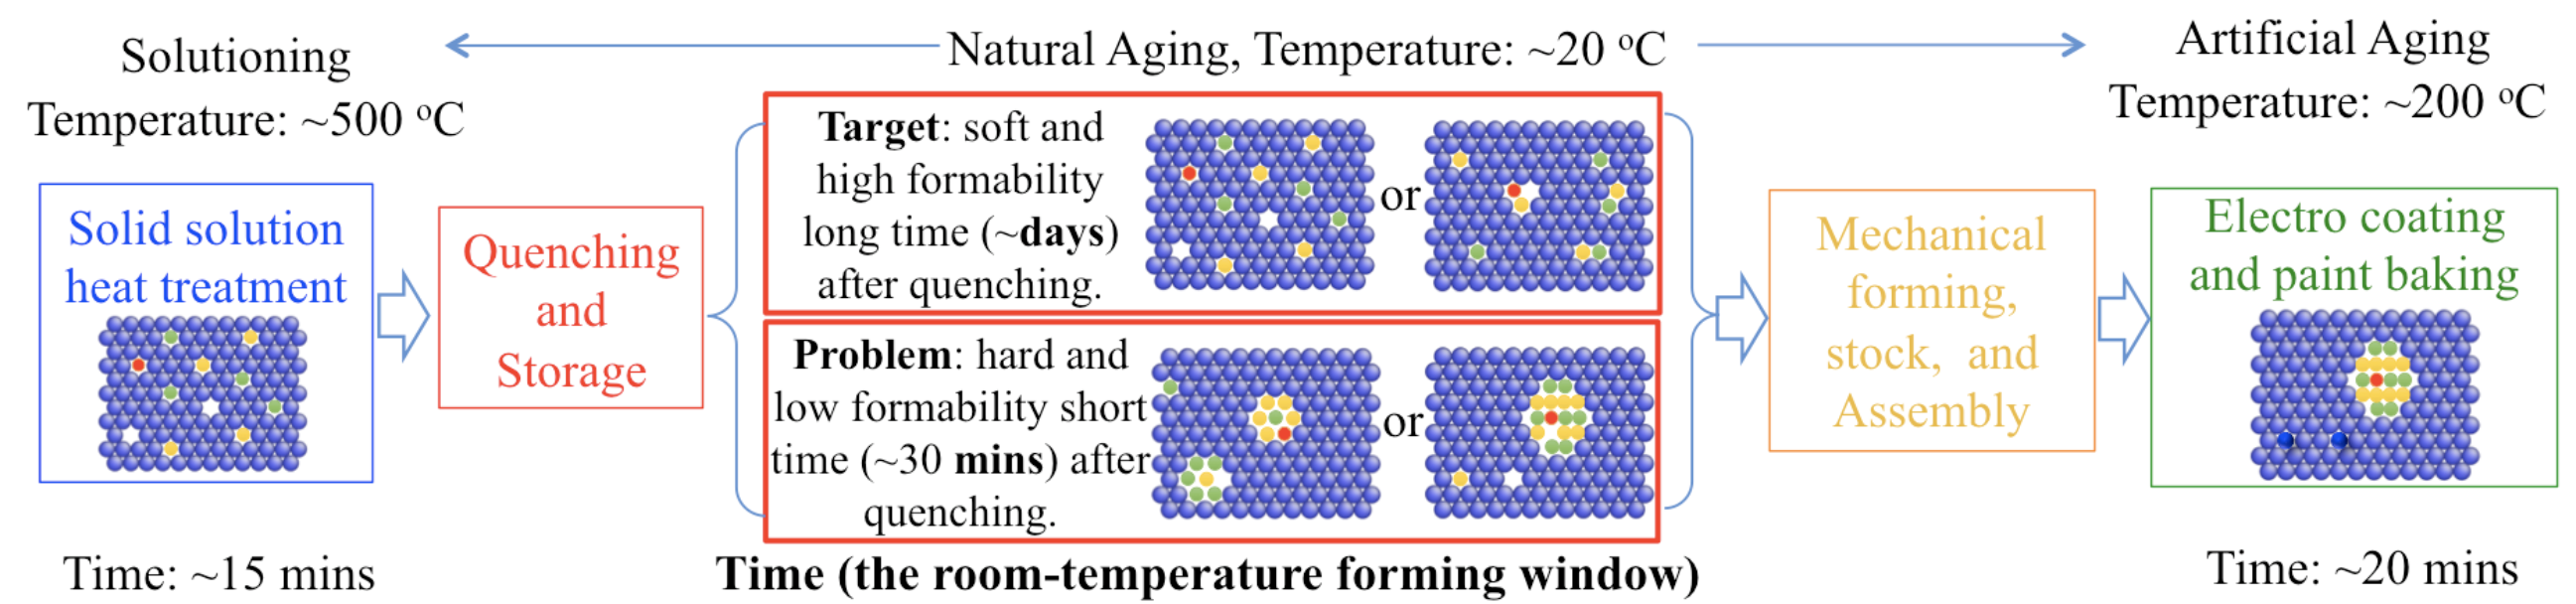
\includegraphics[width=1.0\linewidth]{Chap5/plots/Picture1.png}}
\caption[Schematics of the fabrication process of 7000 series Al sheet alloy parts in the automobile industry.]{Schematics of the fabrication process of 7000 series Al sheet alloy parts in the automobile industry. The corresponding changes of illustrated structures of solute atoms (including clusters and precipitates) during this process are also plotted (blue: Al atoms, other colors: solutes).}
  \label{Chap:Al/Vac:fig1}
\end{figure}
\endgroup

As shown in Figure \ref{Chap:Al/Vac:fig1}, conventional automotive mechanical forming processes, such as stamping and hemming, starts from solid solution heat treatment, then involve room temperature forming of Al sheet alloys in the as-quenched state when alloys have high ductility and formability, and finally followed by artificial aging during the paint bake operation. However, even during the natural aging at room temperatures, the transformation from solid solutions to solute clusters and early-stage precipitates can occur fast  (often within 30 minutes after quenching) for current 7000 series Al alloys. As a result, the formability of these alloys decreases very rapidly and keeps changing as the aging time increases, necessitating costly steps such as warm stamping and coupled solutioning-quenching-stamping operations in a narrow time window\cite{bryant1999effects,li2004biaxial}. These variations of formability and other mechanical properties are all related to the evolution of atomistic structures of precipitates during the sheet processing procedures.

As a result, to understand and to control the nucleation and early stages of precipitation kinetics will have a great impact in automotive applications of age-hardened, light-weight alloys\cite{deschamps1998influence,banhart2011kinetics,liang2012kinetics,deschamps2014precipitation}. The nucleation and growth of precipitates in Al-Zn-Mg-based alloys is currently understood to follow the following sequence: supersaturated solid solution (SSSS) $\rightarrow$ \acf{VRC} $\rightarrow$ \acf{GP} zones (nanoscale coherent Mg/Zn-rich clusters) $\rightarrow$ $\eta'$ (semi-coherent Mg-Zn-Al precipitates with high Zn/Mg ratio) $\rightarrow$ $\eta$ (incoherent $\text{MgZn}_\text{2}$)\cite{ragueneau2000review,deschamps2014precipitation,berg2001gp,chung2018transmission}. During natural aging, the majority of precipitates are \ac{VRC} and \ac{GP} zones, even though $\eta'$ can also be found in some cases\cite{mukhopadhyay1994guinier}. Therefore, in this chapter, how to retard the nucleation and growth of \ac{VRC} and \ac{GP} zones in 7000 series Al alloys during natural aging without adversely affecting the precipitation kinetics during subsequent artificial aging will be focused on. 

Beyond classical theory on the nucleation and early stages of growth of precipitates, atomistic simulations, especially \acf{kMC} simulations, have been applied to investigate the precipitation kinetics in Al alloys\cite{clouet2006kinetic,soisson2010atomistic,soisson1996monte,liang2012kinetics,sha2005kinetic,clouet2004nucleation,vincent2008precipitation,hirosawa1998comparison,sanchez1984generalized}. There simulations were usually conducted to simulate solute atom diffusion based on the vacancy migration in a coherent lattice of the matrix element. Such coherent lattice assumption is still acceptable in our studies of solute clusters and early-stage precipitates. In these \ac{kMC} simulations, the key input is a potential function to describe the activation barrier/energy for the solute/vacancy migration at a particular local lattice occupation environment. For example, the vacancy migration barrier in the pure Al matrix should be different than its counterpart if there is a solute atom occupying the $1^\text{st}$-nearest-neighbor lattice site of the vacancy. Another specific example is shown in Figure \ref{Chap:Al/Vac:barrier}, where the migration barriers for the vacancy jumping to the site \#1, \#2, \#3, and \#4 should be different from each other because these migrations generate distinct change of lattice occupations in the $1^\text{st}$ nearest neighbors of the vacancy.

\begingroup
\begin{figure}[!ht]
  \centering
  \subfigure{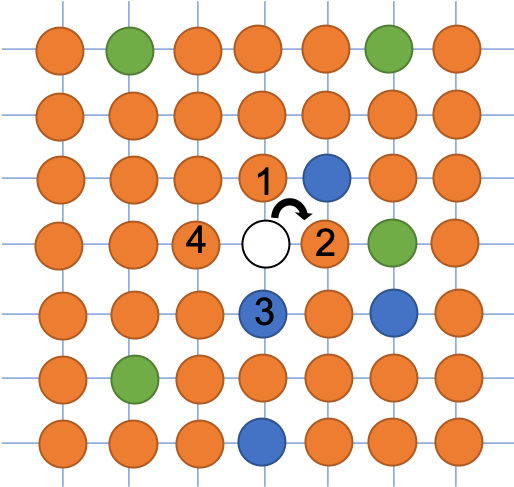
\includegraphics[width=0.5\linewidth]{Chap5/plots/barrier_illustration.png}}
\caption[Illustration of a vacancy migration in a 2D lattice of a multicomponent system.]{Illustration of a vacancy migration in a 2D lattice of a multicomponent system. The orange solid circles represent matrix atoms. Blue and green solid circles represent two different types of solute atoms. The white open circle represents a vacancy. The migration barriers for vacancy jumping to site \#1, \#2, \#3, and \#4 are different based on their $1^\text{st}$ nearest neighbors local environment.}
  \label{Chap:Al/Vac:barrier}
\end{figure}
\endgroup

As we previously mentioned in Section \ref{Chap:Mech:NN}, due to the simplicity of analytical formulas and costly \ac{DFT} calculations, empirical potentials of the vacancy migration barrier usually focus on a limited number of energetic, structural and compositional features in the fitted material systems. As the number of chemical species included in the system increases, it is also getting more difficult to fit the desired empirical potential. For simple vacancy diffusion in bulk lattice or surface diffusion events, \acf{BEP} relationship \cite{bronsted1924katalytische, evans1936further, bell1936theory} was commonly used for calculating the migration barriers of atoms and molecules:
\begin{equation}
\label{Chap:Al/Vac:eq:BEP}
E_a = a \Delta E + b
\end{equation}
where a, b are weighting parameters from fitting, $E_a$ and $\Delta E$ are the migration barrier and the corresponding total energy change due to this migration event, respectively. To further simply the calculations for diffusion in a bulk lattice, researchers used the bond counting model up to a certain cutoff to estimate the total energy change $\Delta E$\cite{soisson1996monte, soisson2010atomistic}. More advanced methods to calculate $\Delta E$ in the coherent lattice include the \acf{CE} formalism that can consider both pair and triple interactions between neighbors \cite{sanchez1984generalized,zunger1994statics,van2001first,persson2010lj,natarajan2016early}. However, most of the \ac{CE} methods only work efficiently for binary or ternary systems due to high computational costs\cite{wu2016cluster}. Even though with some recent development\cite{nguyen2017cluster}, \ac{CE} can predict energy accurately for quinary alloy systems, this method still oversimplified the contribution of atomistic local environments and elastic contributions. Besides, to achieve the same order of accuracy as the number of chemical species increases, the number of parameters needed to fit also increases dramatically\cite{castin2008use}, hence making the computation unaffordable for a long time \ac{kMC} simulations.

Even with correction descriptions of $\Delta E$, we found that the \ac{BEP} relation as Equation \ref{Chap:Al/Vac:eq:BEP} is not valid for the multicomponent alloy systems. As shown in Figure \ref{Chap:Al/Vac:fig2}, the correlation between migration barriers ($E_a$) and energy differences ($\Delta E$) for many vacancy migration events in Al-Mg-Zn systems is far from the linear relation. Here $E_a$ and $\Delta E$ were calculated based on DFT calculations with \acf{CI-NEB}\cite{henkelman2000climbing,henkelman2000improved} in $\sim$1000 cases of vacancy migration in the $4\times4\times4$ supercells of Al fcc lattice with random occupations of Mg/Zn solute atoms. This deviation makes the prediction of accurate vacancy migration barriers very difficult. An inaccurate migration barrier could be fatal in \ac{kMC} models, which is known as the "small-barrier" issue\cite{miron2004multiple}. 


\begingroup
\begin{figure}[!ht]
  \centering
  \subfigure{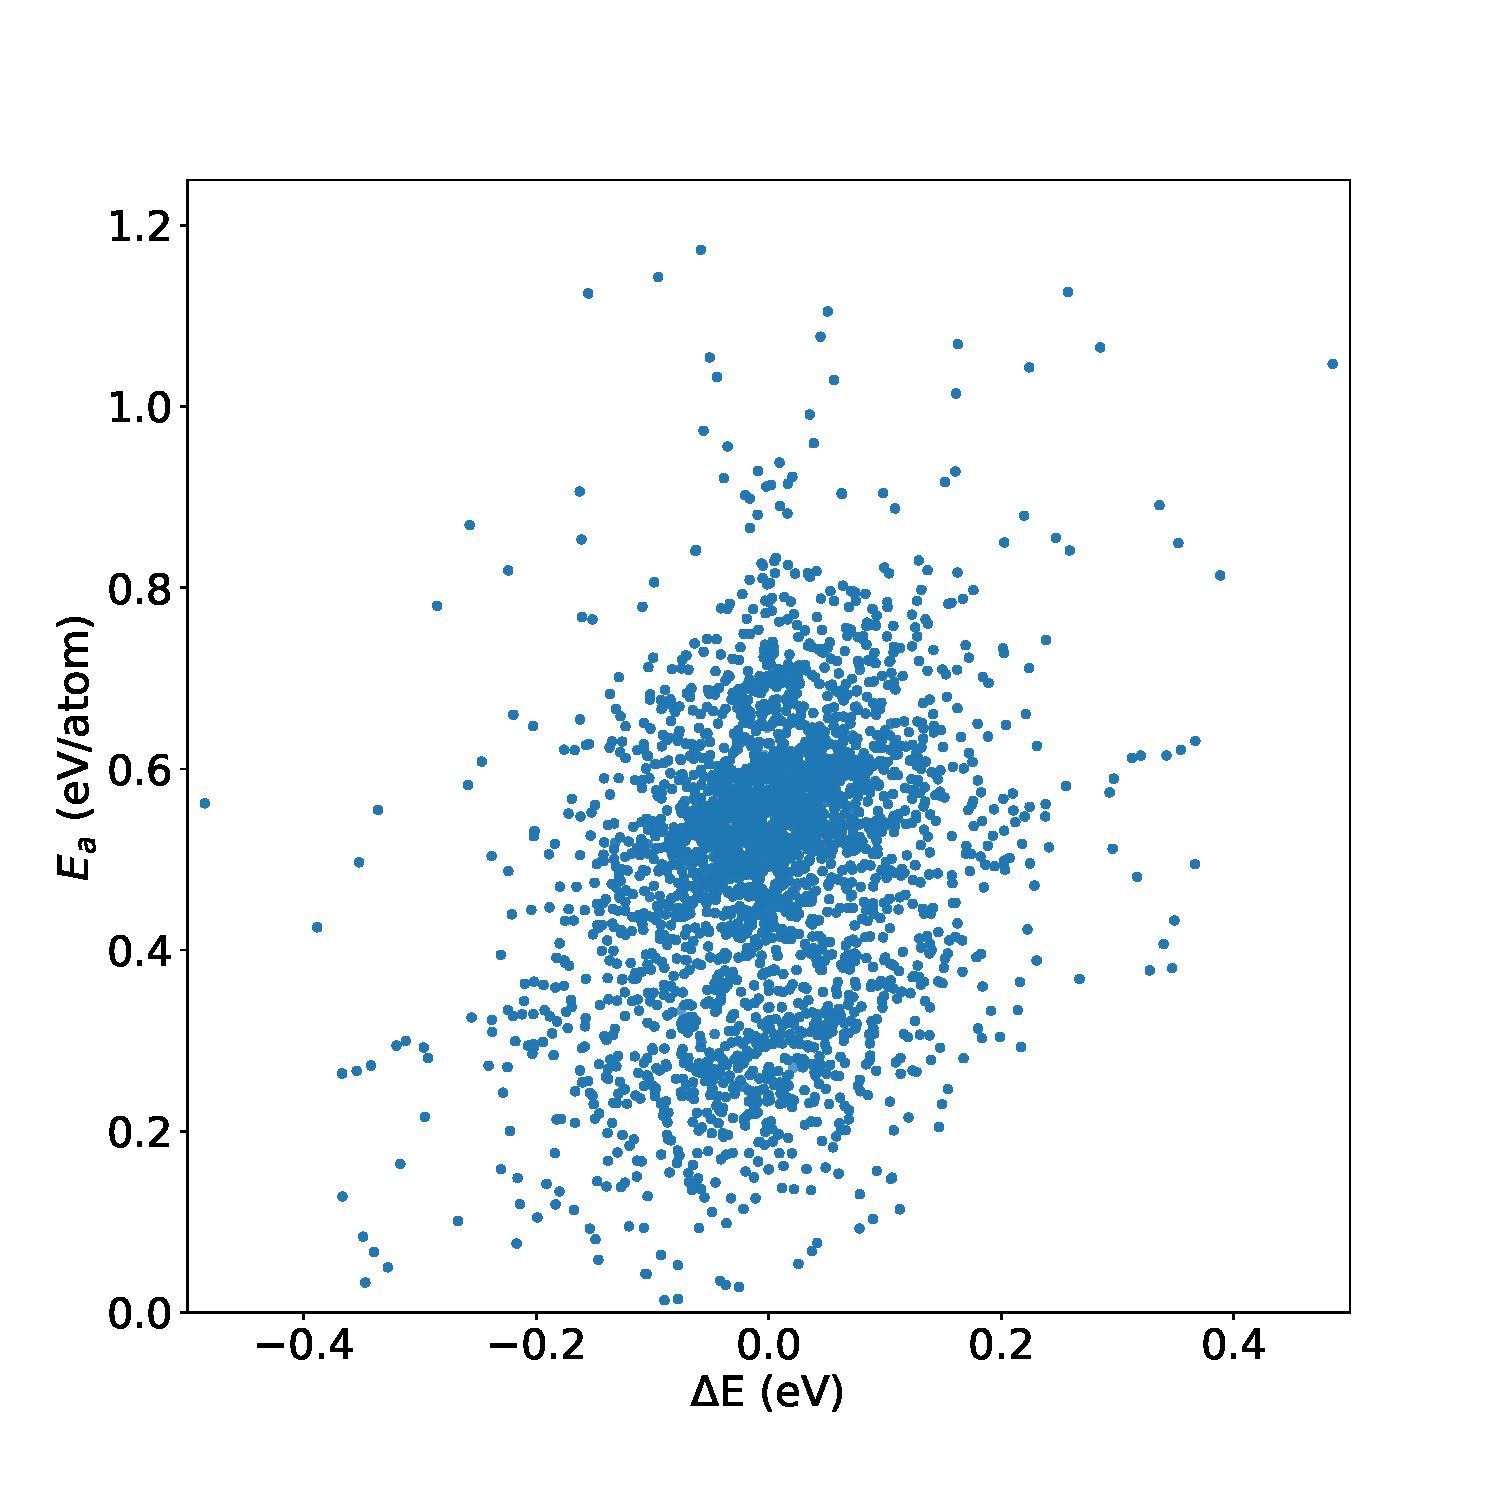
\includegraphics[width=0.8\linewidth]{Chap5/plots/E-EB.pdf}}
\caption[Correlation between migration barriers ($E_a$) and energy differences ($\Delta E$) for many vacancy migration events in Al-Mg-Zn systems obtained from our DFT + \ac{CI-NEB} calculations.]{Correlation between migration barriers ($E_a$) and energy differences ($\Delta E$) for many vacancy migration events in Al-Mg-Zn systems obtained from our DFT + \ac{CI-NEB} calculations.}
  \label{Chap:Al/Vac:fig2}
\end{figure}
\endgroup


Thus, we use a machine learning method to predict accurate vacancy migration barriers for multi-component alloy systems in a coherent fcc lattice. Recently statistical machine learning and artificial intelligence techniques start to be used in many research fields, including materials science and engineering. A typical applications is to use machine learning to construct the numerical functions for the interatomic force fields \cite{bartok2010gaussian,behler2011atom,szlachta2014accuracy,artrith2016implementation,mehta2014exact,artrith2017efficient}. Compared with conventional interatomic potentials with fixed mathematical forms, the high flexibility of these machine-learning methods increase the possibility to fit complex potential energy landscapes with enough accuracy at the level needed. In this work, we develop a \acf{NN} model to predict vacancy migration barriers using the training data set of thousands of \ac{DFT} calculated barriers for different alloy configurations. 


Then, A \ac{kMC} method based on this \ac{NN} model is developed to study the early transition behavior from a supersaturated solid solution to solute clusters and \acf{GP} zones in Al-Mg-Zn alloys. A local super-basin method  \ref{Chap:Al/Vac:sec:LSKMC}, together with \ac{LRU} cache \ref{Chap:Al/Vac:sec:LRU}, is also implemented to accelerate \ac{kMC} simulations. We also propose a pseudo-atoms approach to efficiently search the alloying strategy to slow down the solute clustering and the corresponding natural aging effects in Al 7000 series alloys. We also develop the quantitative analysis methods to describe the chemical and structural properties of clusters. At last, we propose a machine learning strategy based on the structural and chemical information of clusters and precipitates from \ac{kMC} simulations to predict the cluster strengthening and natural aging effects in future studies.
\section{Fitting Diffusion Barriers using Neural Network}
\label{Chap:Al/Vac:section:NN}

The computational engine that provided the energetics used to evaluate energy differences and activation barriers before and after vacancy jump in Al 7075 alloy was the implementation of \ac{DFT} together with climbing image \acf{NEB} in the \ac{VASP} software with VTST package from Henkelman's group \cite{henkelman2000climbing,henkelman2000improved}. All-electron \ac{PAW} potentials were employed for the elemental constituents with the \ac{GGA} of \ac{PBE} for the exchange-correlation energy functional, $\mu_{xc}$, and the interpolation formula of Vosko et al. \cite{vosko1980accurate}. Using plane-wave cutoff energy of at 450.0 eV, the total energy for all models of initial and final images was converged to $10^{−7}$ eV/cell. The reciprocal space of bulk supercells was sampled with (2x2x2) k-point grids. Each grid was generated using the Monkhorst-Pack scheme \cite{monkhorst1976special}. A (4x4x4) conventional supercell with a single vacancy embedded was used for these calculations. For activation barrier calculations, 5 images between relaxed initial and final images were used. A spring constant was set to 5 $\text{eV}/\angstrom^2$. The force convergence criteria for all models was set to be less than 0.05 $\text{eV}/\angstrom$. The force-based quick-min optimizer was used to make \ac{NEB} calculations stable for high local concentration cases. \cite{sheppard2008optimization}


We calculated lattice constant for Al 7075 alloy, using \acfp{SQS} method \cite{zunger1990special}. A (4x4x4) conventional supercell with 256 atoms was used. The types of 256 atom was chosen to be 244 Al atoms, 7 Mg atoms, and 5 Zn atoms, which is within the concentration range of Al 7075 alloy. The obtained lattice constant is 4.05838 \angstrom, which is roughly the lattice constant (4.041\angstrom) of pure Al.


To sample a larger potential energy landscape, our \ac{NN} model training set contains mainly two different parts, as shown in Fig. \ref{Chap:Al/Vac:fig:atomic_illu}: 1) (4x4x4) randomly generated solid-solution structures with different local concentrations around jump pairs. 2) (2x2x2) randomly generated ordered structures embedded in (4x4x4) pure Al. The first training set is good for simulating vacancy diffusion of a very early stage, during which Al alloy is in the solid-solution state. The second training set is designed to accurately describe the behavior of vacancy moving across/along the boundary between solid-solution Al and ordered phases, and moving inside the ordered phases. The atomic structures of ordered phases are chosen from proposed GP zone structures from \cite{berg2001gp} and low energy ordered $\text{L1}_\text{0}, \text{L1}_\text{2}, \text{L1}_\text{0}^*, \text{W2}, \text{CH}, \text{L1}_\text{2}^*, \text{Z1}$ structures of Au-Fe from \cite{zhuravlev2017phase} with random species perturbation. The atomic  structures were generated using our in-house code KNN2. \cite{Zhang2020KNN2}


\begingroup
\begin{figure}[!ht]
  \centering
  \subfigure[]{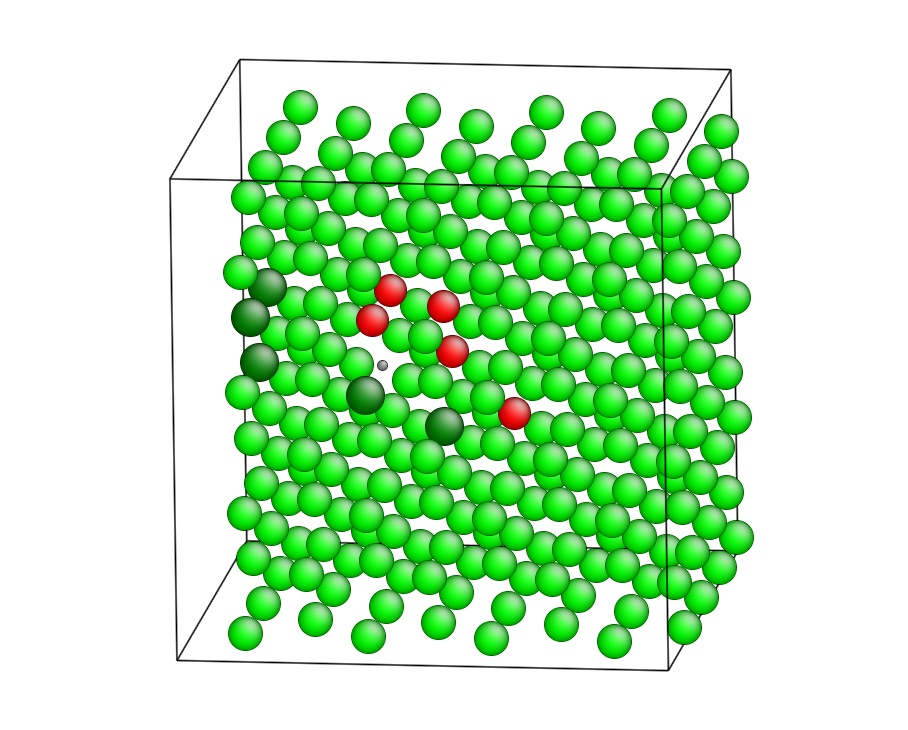
\includegraphics[width=0.49\linewidth]{Chap5/plots/ss_atomic.jpg}}
  \subfigure[]{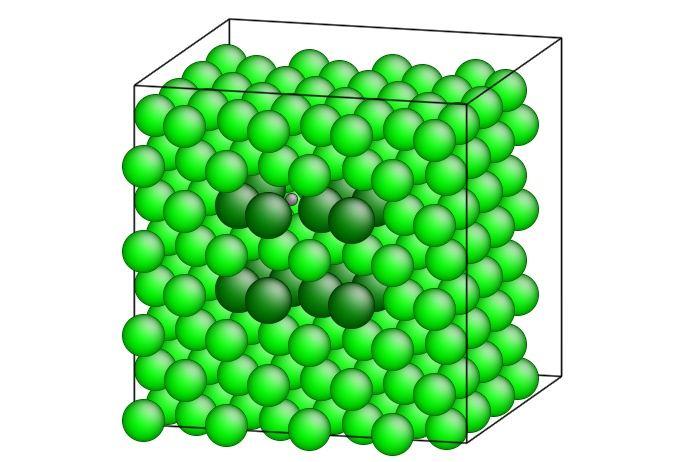
\includegraphics[width=0.49\linewidth]{Chap5/plots/ordered_atomic.jpg}}
\caption[Atomistic pictures of (4x4x4) supercells containing 256 atoms.]{Atomistic pictures of (4x4x4) supercells containing 256 atoms. (a) One typical (4x4x4) randomly generated solid-solution structure. (b) One typical (2x2x2) randomly generated ordered structures embedded in (4x4x4) pure Al. Light green, dark green, and red atoms are Al, Mg, and Zn, respectively. The small gray atom represents the location of vacancy.}
\label{Chap:Al/Vac:fig:atomic_illu}
\end{figure}
\endgroup


Many different machine learning/deep learning models are widely used, each one suitable for a different kind of problem. \cite{bartok2010gaussian,behler2011atom,szlachta2014accuracy,artrith2016implementation,mehta2014exact,artrith2017efficient} For our particular problem, the feed-forward Artificial Neural Network (ANN) is chosen, as it provides a general frame to map non-linear input (atomic species of neighboring environment) to a continuous regressor (diffusion barriers). It is well known that a sufficiently large number of hidden neurons can approximate any continuous multivariate function. \cite{hornik1989multilayer} This property gives us the most expandability of this framework when the system needs to go even further complicated in terms of the number of species considered. 


The output layer of our \ac{NN} model predicts diffusion barriers in a 1-D continuous space. The input layer was chosen to be 27 discrete numbers representing atom species based on Ising model, as shown in Table. \ref{Chap:Al/Vac:tab:mapping}. Among the 27 numbers, the first one indicates the type of atom that will be swap with the vacancy. The rest 26 (each atom has 12 + 6 = 18 $\text{2}^{nd}$ nearest neighbors. And both of them share 10 in common.) atoms represents the neighboring atoms of the jump pair up to their $\text{2}^{nd}$ nearest neighbors, as shown in Fig. \ref{Chap:Al/Vac:fig:2nn}. The rest 26 numbers are arranged in their geographical order (ascending in X, Y, and Z accordingly), so their position will always respond to the same input neuron in the \ac{NN} architecture. Besides, this cluster of 26 neighboring atoms also has 2-fold symmetry, mirror symmetry along Y-Z plane, and mirror symmetry along the X-Y plane. Therefore, for one jumping event, the diffusion barrier is taken as the average of the four symmetric configurations of the 26 neighboring atoms to have a rotation-invariant prediction. By using several layers of hidden neurons between 27 input species and 1 output diffusion barrier, the contribution distribution to final output, diffusion barrier, of pair-wise and triple-wise interactions can be learned.


\begin{table}[!htbp]
\centering
\caption[Atom species encoding map for the \acf{NN} input layer.]{Atom species encoding map for the \acf{NN} input layer. Here, ``Vac'' represents vacancies.}
\label{Chap:Al/Vac:tab:mapping}
\begin{tabular}{ll}
\\
\hline
\hline
Species & Encoding  \\ \hline
Al & 1.0 \\
Mg & 2.0 \\
Zn & 3.0 \\
Vac & 4.0 \\
\hline
\hline
\end{tabular}
\end{table}


\begingroup
\begin{figure}[!ht]
  \centering
  \subfigure{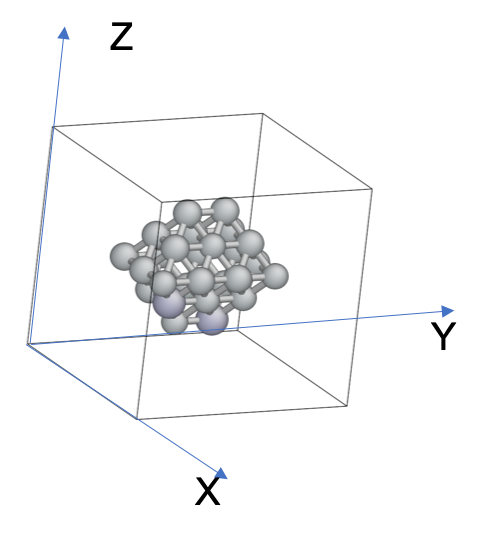
\includegraphics[width=0.5\linewidth]{Chap5/plots/2nn.png}}
\caption[Illustration of atomic structures of the $\text{2}^{nd}$ nearest neighbors surrounding the jumping pairs.]{Illustration of atomic structures of the $\text{2}^{nd}$ nearest neighbors surrounding the jumping pairs. The 26 neighboring atoms have 2-fold symmetry, mirror symmetry along Y-Z plane, and mirror symmetry along the X-Y plane.}
\label{Chap:Al/Vac:fig:2nn}
\end{figure}
\endgroup


We implemented the \ac{NN} model using Google's TensorFlow \cite{abadi2016tensorflow} with Keras \cite{chollet2015keras}. TensorFlow is an open source numerical computation framework using data flow graphs with the ability of deriving gradients automatically. Keras is a high-level neural networks API, written in Python and capable of running on top of TensorFlow. The optimized neural network structures was tuned by Talos \cite{Autonomio2019Talos}. The Adam optimizer \cite{kingma2014adam} was used for optimizing weights in the neural network. Xavier uniform initializer \cite{glorot2010understanding} was used to generate the random weights and biases so as to break the symmetry of weighting parameters. The activation functions were chosen to be \acf{ReLu}. The optimized \ac{NN} architecture can be found in Table. \ref{Chap:Al/Vac:tab:NN}.


\begin{table}[!htbp]
\centering
\caption[Neural network architecture with activation functions and dropout probability of each layer.]{Neural network architecture with activation functions and dropout probability of each layer.}
\label{Chap:Al/Vac:tab:NN}
\begin{tabular}{cccc}
\\
\hline
\hline
Layer & Shape  & Activation  & Dropout Probability\\ 
\hline
Dense & 256    & ReLu       & 0.1                 \\
Dense & 256    & ReLu       & 0.2                 \\
Dense & 128    & ReLu       & 0.0                 \\
Dense & 64     & ReLu       & 0.05                \\
Dense & 64     & ReLu       & 0.0                 \\
Dense & 16     & ReLu       & 0.0                 \\
Dense & 1      & Linear     & N.A.                \\ 
\hline
\hline
\end{tabular}
\end{table}


To train the \ac{NN}, two different loss functions are used. The former one is the common \acf{MSE} via:
\begin{subequations}
\begin{align}
MSE = \frac{1}{N}\sum_{i=1}^{N}({E_a}_{i}^{DFT} - {E_a}_{i}^{NN})^2
\label{Chap:Al/Vac:eq:MSE}
\end{align}
\end{subequations}
where $N$ is the number of input datas, which can be trained in batch or mini-batch, ${E_a}_i^{DFT}$ is the diffusion barrier of $i^{\text{th}}$ data from \ac{DFT} calculation, and ${E_a}_{i}^{NN}$ is from \ac{NN} prediction. As shown in Fig. \ref{Chap:Al/Vac:fig:fitting_all}, the model reached a \ac{RMSE} of 0.04313 eV/atom for all the data points. The latter one is a customized loss function, via:
\begin{subequations}
\begin{align}
Loss = \frac{1}{N}\sum_{i=1}^{N}{(1.0 + \alpha (1.5 - {E_a}_{i}^{DFT})({E_a}_{i}^{DFT} - {E_a}_{i}^{NN})^2)}
\label{Chap:Al/Vac:eq:custLoss}
\end{align}
\end{subequations}
where $\alpha$ is a tunable knob. A larger $\alpha$ value will weigh more on diffusion barriers that are small. In this way, we are able to fit low-energy barriers more accurately, as they are the critical rate-determining steps in a \ac{KMC} simulation. Using this custom loss function, the model reached a \ac{RMSE} of 0.03785 eV/atom for all the data points. Noting that the model trained using the latter loss function is slightly more accurate than the former method because more data points are located far away from 1.5 eV. As we expected, low-energy barriers are predicted with higher accuracy, which can be seen from Fig. \ref{Chap:Al/Vac:fig:fitting_all_weighted}.


\begingroup
\begin{figure}[!ht]
  \centering
  \subfigure[]{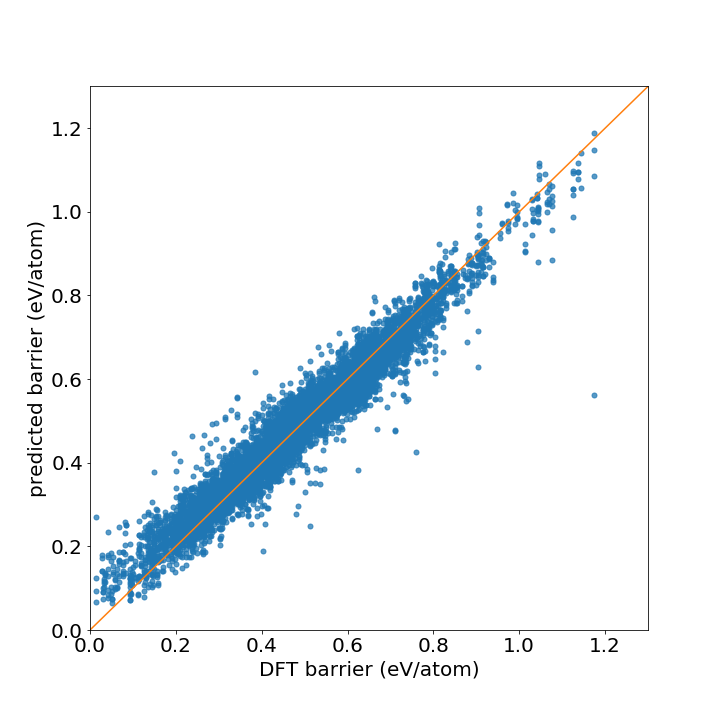
\includegraphics[width=0.49\linewidth]{Chap5/plots/total.png}}
  \subfigure[]{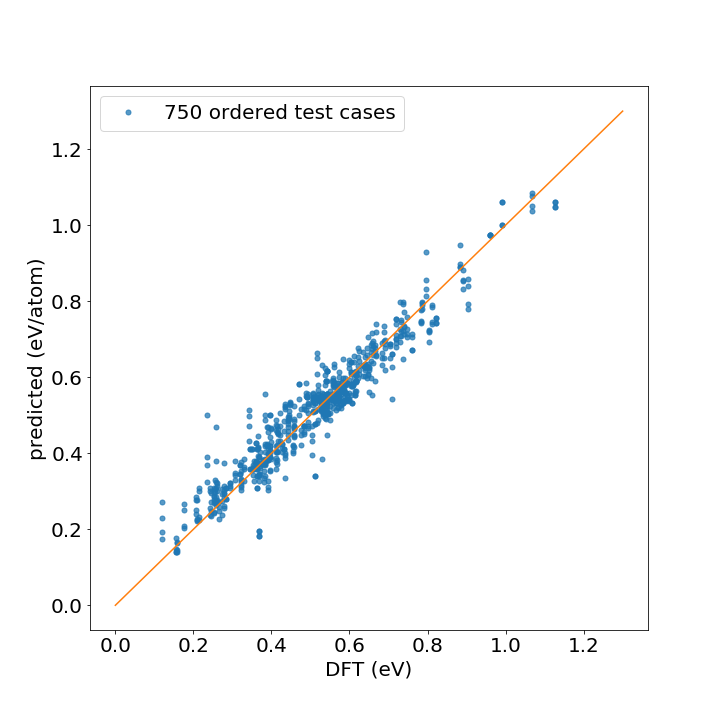
\includegraphics[width=0.49\linewidth]{Chap5/plots/fit_ordered.png}}
\caption[Predictions accuracy of diffusion barriers from neural network surrogate model, compared with DFT calculated results.]{Predictions accuracy of diffusion barriers from neural network surrogate model, compared with DFT calculated results. The orange solid line indicates perfect fitting. Each blue solid dot represents one data point. (a) predictions of all the barriers. (b) predictions of teneray ordered structures.}
\label{Chap:Al/Vac:fig:fitting_all}
\end{figure}
\endgroup

\begingroup
\begin{figure}[!ht]
  \centering
  \subfigure[]{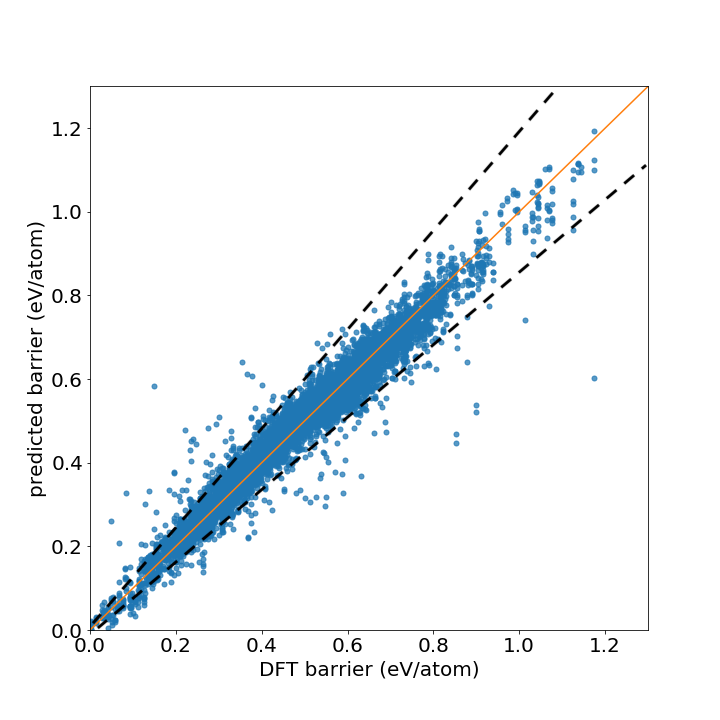
\includegraphics[width=0.49\linewidth]{Chap5/plots/total_weighted.png}}
  \subfigure[]{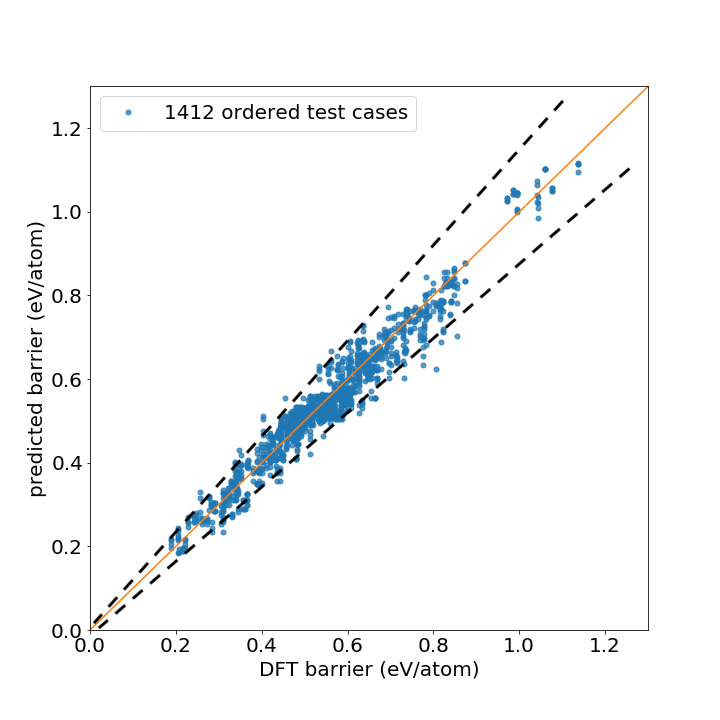
\includegraphics[width=0.49\linewidth]{Chap5/plots/fit_ordered_weighted.png}}
\caption[Predictions accuracy of diffusion barriers from neural network model using custom loss function, compared with DFT calculated results.]{Predictions accuracy of diffusion barriers from neural network model using custom loss function, compared with DFT calculated results. During model training, eq. \ref{Chap:Al/Vac:eq:custLoss} was used to weigh more on low-energy barriers. The orange solid line indicates perfect fitting. Each blue solid dot represents one data point. The black dashed lines illustrate the confinement introduced by custom loss function with emphasis on low-energy-barrier data points. (a) predictions of all the barriers. (b) predictions of ternary ordered structures.}
\label{Chap:Al/Vac:fig:fitting_all_weighted}
\end{figure}
\endgroup
\section{Kinetic Monte Carlo Setup}
\label{Chap:Al/Vac:section:KMC}

\newpage
\begingroup
\begin{figure}[!ht]
  \centering
  \subfigure{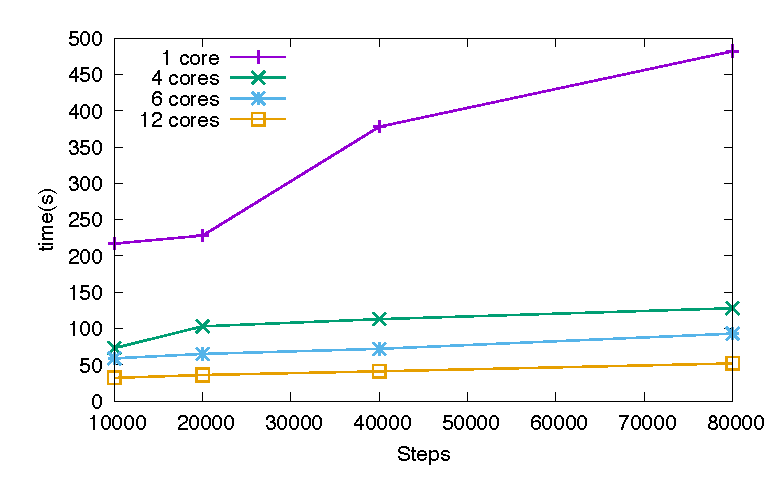
\includegraphics[width=1.0\linewidth]{Chap5/plots/scale.eps}}
\caption[Scalability of KNN2 code on Great Lakes HPC.]{Scalability of KNN2 code for 108,000 atoms on Great Lakes HPC from the University of Michigan with 2x 3.0 GHz Intel Xeon Gold 6154 processors and InfiniBand HDR100 networking, capable of 100 Gb/s throughput.}
\label{Chap:Al/Vac:fig:scale}
\end{figure}
\endgroup

\section{Results and Discussion}
\label{Chap:Al/Vac:section:RD}
\subsection{Cluster Searching Algorithm}

In order to better analyzing our results, we have to use a visualization method to characterize clusters. A cluster is a set of connected atoms, each of which is within the range of one or more other atoms from the same cluster. Thus, any two atoms from the same cluster are connected by a continuous path consisting of steps fulfilling the selected neighboring criterion. Adversely, two atoms are not considered in the same cluster if there is no continuous path on the neighbor network leading from one particle to the other. We choose between the distance-based neighbor criterion, in which case two atoms are considered neighbors if they are within the neighbor list of each other. However, in our case, all the atoms are on lattice, so the method described above does not work. It will simply find one huge cluster containing all the atoms. Therefore, we use the method described in Algorithm. \ref{algo:cluster}. We show one typical results in Fig. \ref{Chap:Al/Vac:fig:illu_cluster}. The only top ten clusters are shown. And as you can see, dark red and orange clusters are almost connected. They share one Al atom in common. In that case we treat them as two clusters. Otherwise, if Al atoms are treated like bridges, then most of the atoms in the supercell will be connected as one huge cluster, which is not desired.


\begin{figure}[!htb]
  \centering
  \begin{minipage}{.75\linewidth}
    \begin{algorithm}[H]
      \caption{Cluster Searching Algorithm}\label{algo:cluster}
      \begin{algorithmic}[1]
        \State remove all the solvent atoms (Al for example).
        \State assign an initial cluster id, ($cid = -1$), to all the atoms.
        \State set $count = 0$.
        \For {i in all the solute atoms}
          \If {$cid_i = -1$}
            \State set $cid_i = count$.
            \State \ac{BFS} in the neighbor list of atom i to find other solute atoms if cluster size is greater than $size_{critical}$ and set their $cid = count$.
            \State add their first nearest neighbor solvent atoms (Al for example) back if the solvent atom have more than $bond_{critical}$ solute first nearest neighbors and set their $cid = count$.
            \State $count += 1$.
          \EndIf
        \EndFor
        \State then clusters can be sorted according to any customized methods, by cluster size, element ratios for examples.
      \end{algorithmic}
    \end{algorithm}
  \end{minipage}
\end{figure}


\begingroup
\begin{figure}[!ht]
  \centering
  \subfigure[]{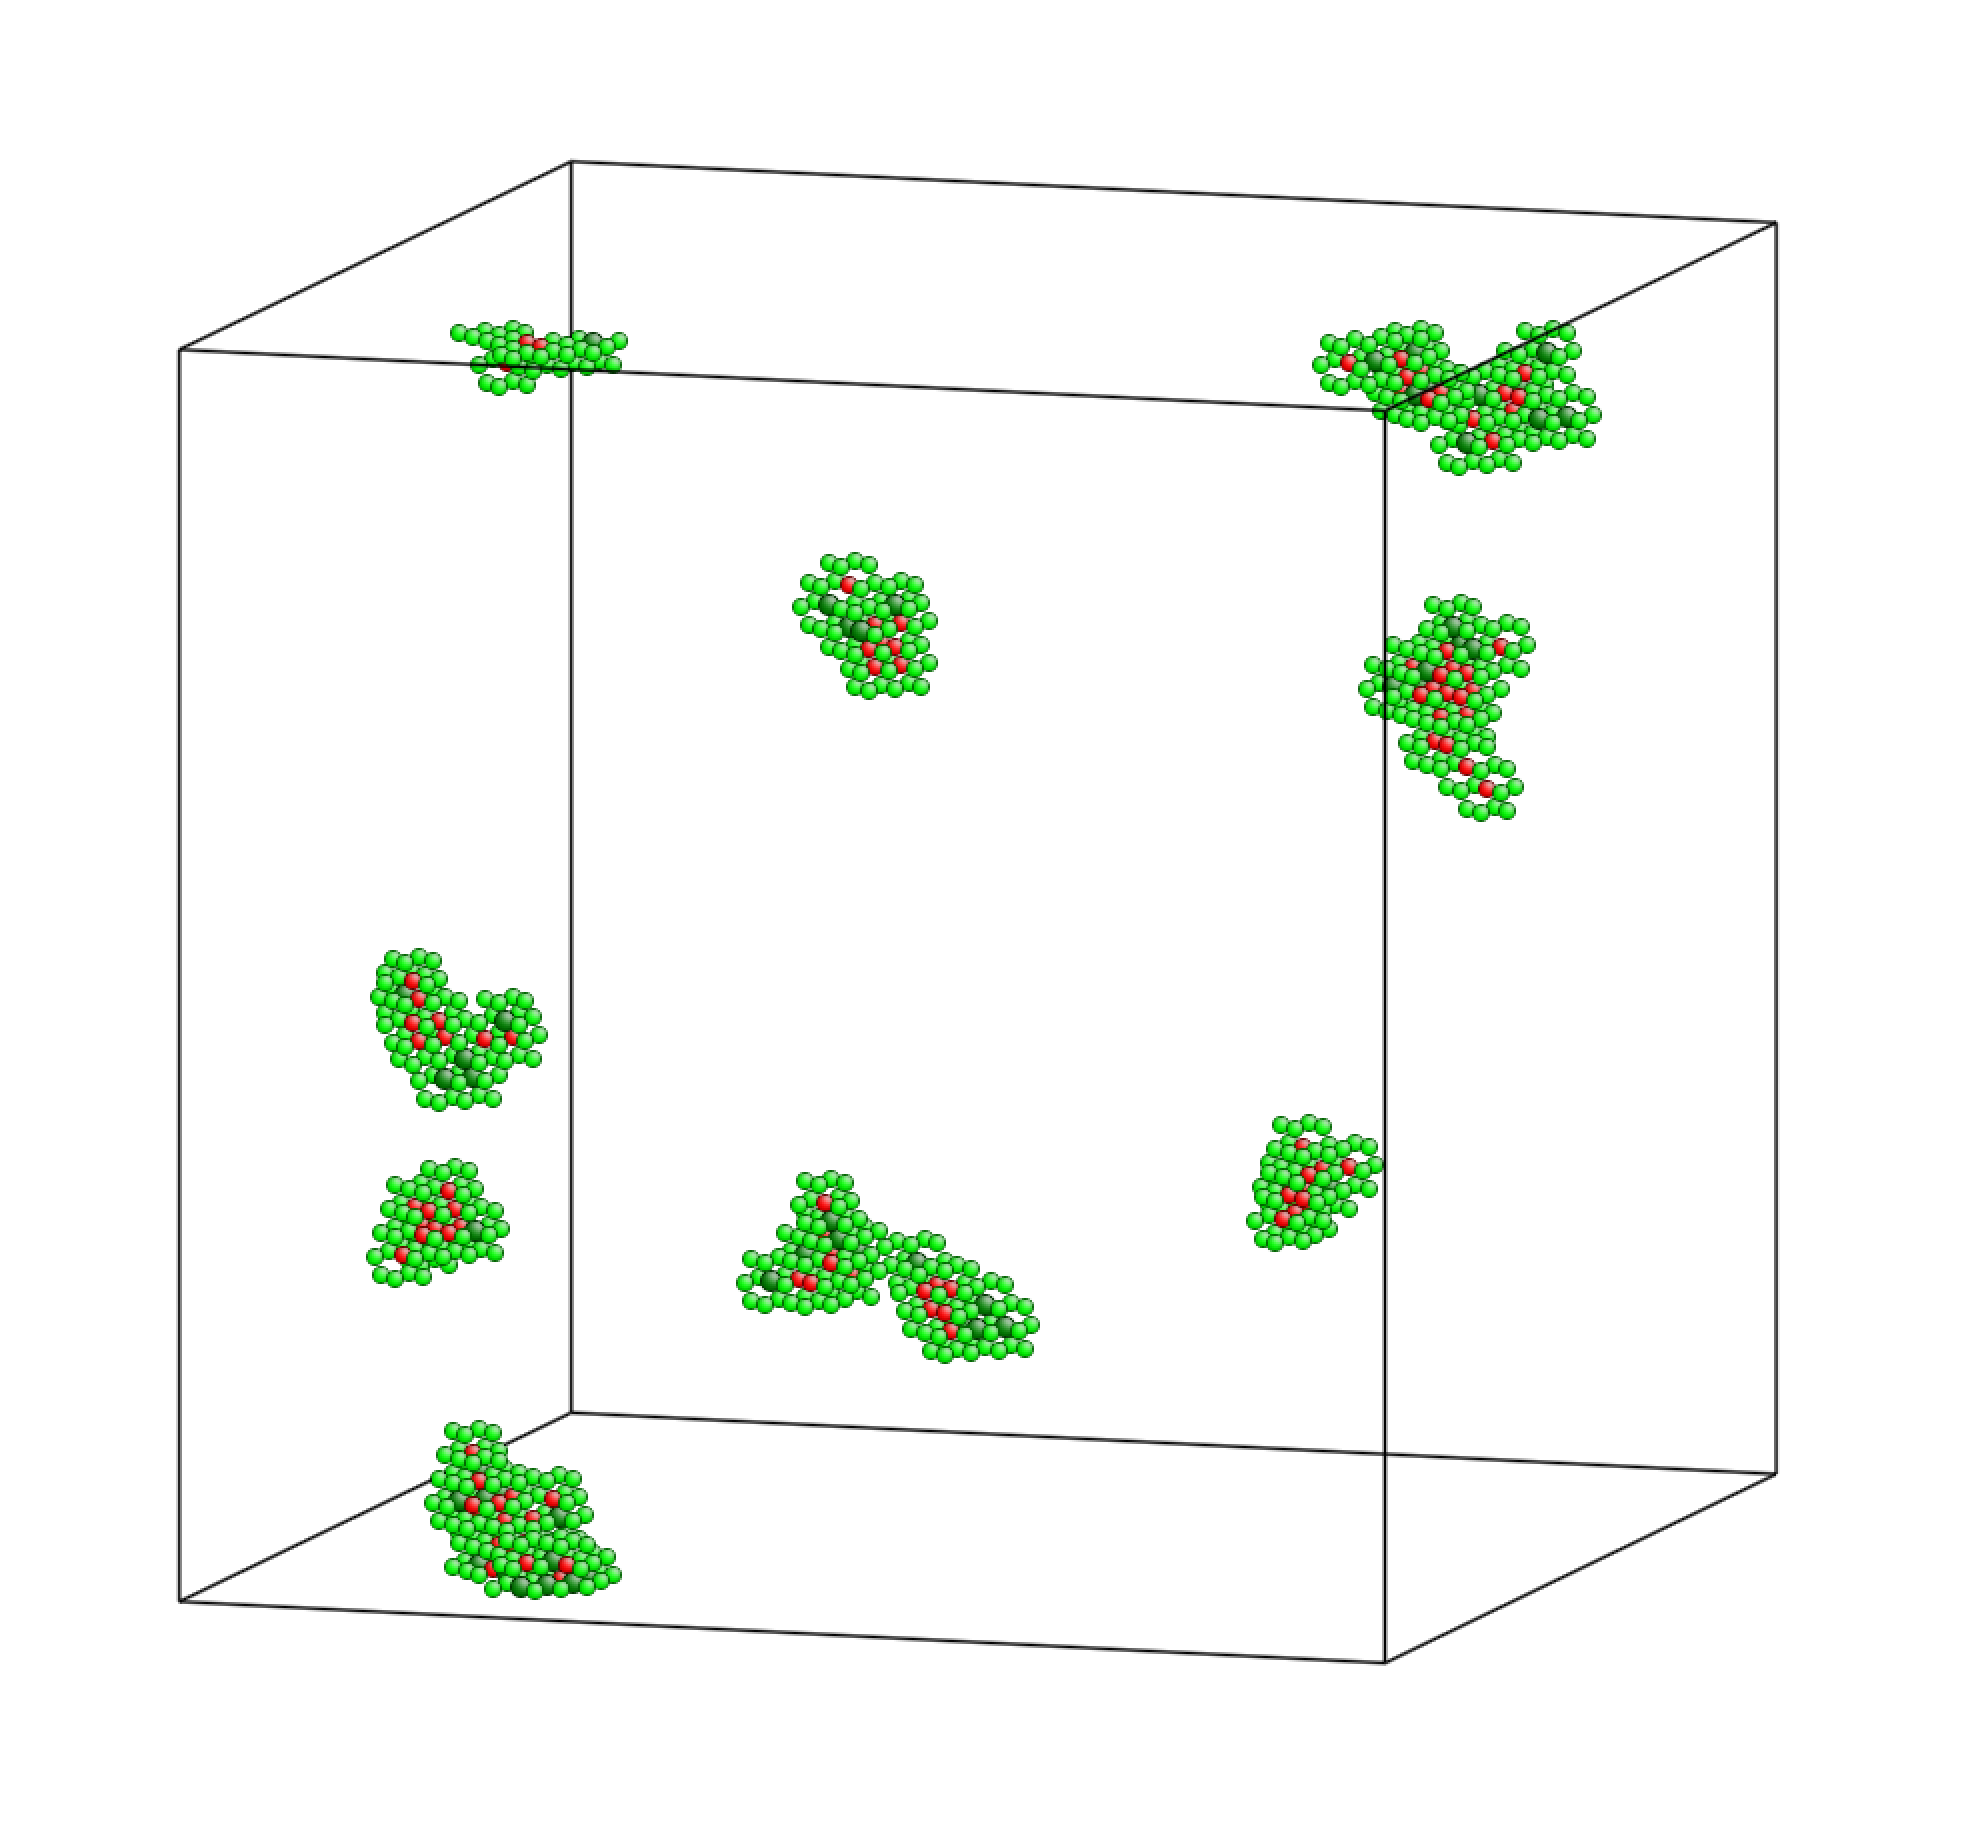
\includegraphics[width=0.49\linewidth]{Chap5/plots/cluster_illu_1.png}}
  \subfigure[]{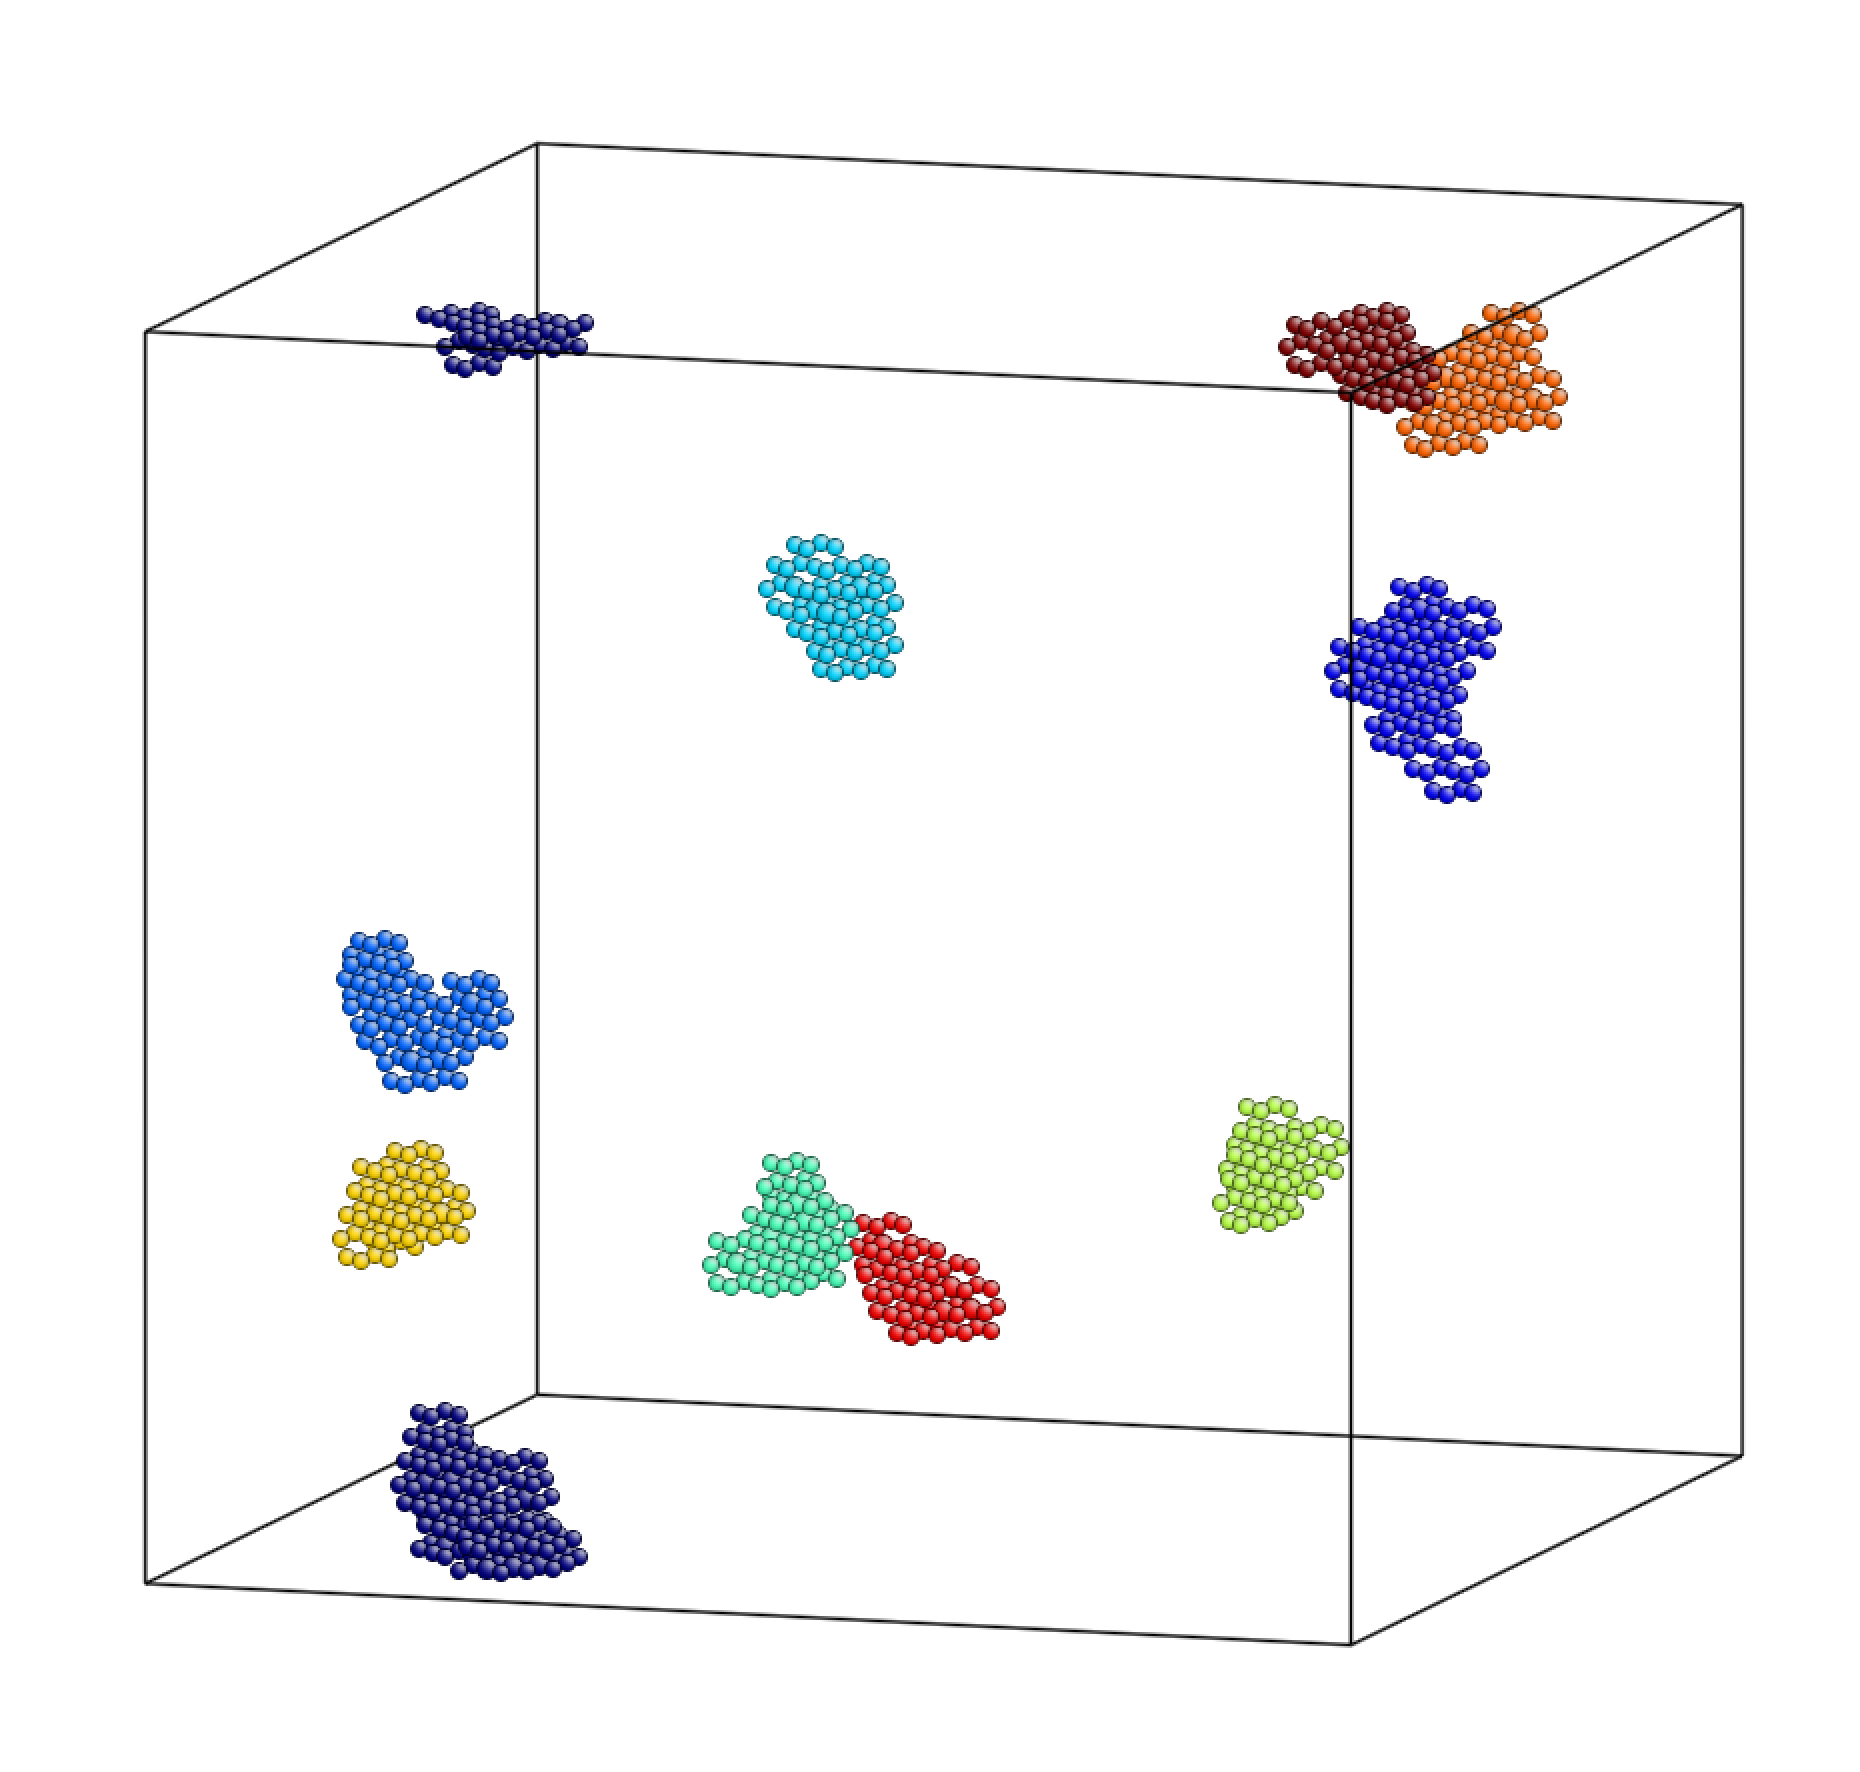
\includegraphics[width=0.45\linewidth]{Chap5/plots/cluster_illu_2.png}}
\caption[Atomistic pictures of top 10 clusters by size via cluster searching algorithm.]{Atomistic pictures of top 10 clusters by size via cluster searching algorithm. (a) Atomistic pictures of clusters coloring in atom species. Light green, dark green, and red atoms are Al, Mg, and Zn, respectively. (b) Atomistic pictures of clusters coloring in cluster id. The color mapping from dark blue to red is ranked by the cluster size in descending order.}
\label{Chap:Al/Vac:fig:illu_cluster}
\end{figure}
\endgroup


\subsection{Searching for Potential Elements that Can Slow Down Early Stage Nucleation}
\label{Chap:Al/Vac:pseudo}
Similar to the idea of searching ``anchor'' elements in Chap. \ref{Chap:Ag/ZnO:section:anchor}, we will first use \ac{KMC} simulation with some pseudo-atoms (denoted as ``X'') to study their effects on the early stage clustering. In this study, we have Al atoms as solvent atoms, and Mg, Zn atoms as solute atoms. To tune the properties of pseudo atoms, we can change the effects of different elements on vacancy diffusion barriers to the pseudo-atoms, as well as barriers to other elements. We leverage this by adding an offset to the diffusion barrier calculated from \ac{NN} model via Equation. \ref{Chap:Al/Vac:eq:offset} . The amount of the offset is determined by counting first neighbor bonding of X-Al, X-Mg, and X-Zn, via Equation. \ref{Chap:Al/Vac:eq:offset_calculation}:
\begin{subequations}
\begin{align}
{E_a}^{actual} & = {E_a}^{NN} + \textit{offset} \label{Chap:Al/Vac:eq:offset} \\
\textit{offset} & = \sum_{i\in\{Al, Mg, Zn\}} \varepsilon_{i-X} * ( n_{i-X}^{final} - n_{i-X}^{init}) \label{Chap:Al/Vac:eq:offset_calculation}
\end{align}
\end{subequations}
where ${E_a}^{NN}$ is the energy obtained by the neural network prediction of treating element ``X'' as the solvent element Al, the summation is confined to first nearest-neighbors of the vacancy and of the jumping atom, $\varepsilon_{i-X}$ represents the amount of different pairs' effects on the diffusion barrier offset, and $n_{i-X}$ is the number of first nearest neighbor $i-X$ pairs. For example, if $\varepsilon_{Al-X} = 0.01$ that means increasing an Al-X pair will increase the diffusion barrier by a positive 0.01 eV.


The right hand side of Equation. \ref{Chap:Al/Vac:eq:offset} can be divided into two parts. The first part, which is \ac{NN} potential part, can be seen as a more comprehensive bond counting model \cite{soisson1996monte} base on the pair interactions of Al-Al, Al-Mg, Al-Zn, and Mg-Zn, plus cross interactions or higher odered angular contributions. And the second part of the RHS is can be seen as first order bond counting of Al-X, Mg-X, and Zn-X. As a qualitative study, first order pair-wise interaction of the unknown pseudo-atoms should be sufficient. If we rearrange Equation. \ref{Chap:Al/Vac:eq:offset}, we will have:
\begin{subequations}
\begin{align}
{E_a}^{actual} & = \sum_{i, j \in\{Al, Mg, Zn, X\} \& i \neq j} \varepsilon_{i-j} * ( n_{i-j}^{final} - n_{i-j}^{init}) + \textit{H.O.T.(Al, Mg, Zn)} \label{Chap:Al/Vac:eq:rearrange}
\end{align}
\end{subequations}
where $H.O.T$ is the higher order term, such as bond angles. Then the target is to find an element ``X'' that can change the diffusion barrier of Vac-i by roughly the amount of $\varepsilon_{i-X}$, where $i \in \{Al, Mg, Zn\}$.


\begin{table}[!htbp]
\centering
\caption[Sensitivity analysis of different $\varepsilon_{i-X}$.]{Sensitivity analysis of different $\varepsilon_{i-X}$. In the table, the number of different element types are listed using $size_{critical}$ of 3(4) and $bond_{critical}$ of 3(4).}
\label{Chap:Al/Vac:tab:pseudo1}
\begin{tabular}{cccccccc}
\\
\hline
\hline
setup & $\varepsilon_{Al-X}$  & $\varepsilon_{Mg-X}$  & $\varepsilon_{Zn-X}$ & Al counts & Mg counts & Zn counts & pseudo counts\\
\hline
0 &  0.00    &  0.00       &  0.00 & 1078(230) & 588(421)  &  737(524)  & 11(4)                \\
1 &  0.05    &  0.00       &  0.00 & 1229(270) &  689(434) &   778(549) & 0(0)                \\
2 & -0.05    &  0.00       &  0.00 & 1407(312) & 922(753)  & 1017(871)  & 406(252)                \\
3 &  0.05    &  0.05       &  0.00 & 1442(353) & 1121(919) & 794(620)   & 292(171)                \\
4 &  0.00    & -0.05       &  0.00 & 1012(215) &  588(407) &  638(463)  & 5(1)                \\
5 &  0.00    &  0.00       &  0.05 & 1407(395) & 522(407)  & 1325(1164) & 385(253)                \\
6 &  0.00    &  0.00       & -0.05 & 1042(222) &  590(363) &  730(489)  & 3(0)                \\

\hline
\hline
\end{tabular}
\end{table}


To setup the simulation for sensitivity tests, we use \ac{LSKMC} method with $step_{critical}$ of 25,000 steps and $E_{critical}$ of 0.3 eV. After around 5 $\sim$ 6 seconds simulation, we can already tell the differences of cluster size obviously. As discussed above, we tuned parameters of $\varepsilon_{i-X}$ for $i \in {Al, Mg, Zn}$. Detailed setup is listed in Table. \ref{Chap:Al/Vac:tab:pseudo1}. And their corresponding final snapshots can be found in Fig. \ref{Chap:Al/Vac:fig:sens_Al}, Fig. \ref{Chap:Al/Vac:fig:sens_Mg}, and Fig. \ref{Chap:Al/Vac:fig:sens_Zn}, respectively. In order to achieve the target of finding a suitable element ``X'', we can use \ac{DFT} with \ac{NEB} to search for elements that can change the diffusion barrier of Vac-i by roughly the amount of $\varepsilon_{i-X}$, where $i \in \{Al, Mg, Zn\}$.


\newpage
\begingroup
\begin{figure}[!ht]
  \centering
  \subfigure[Al Mg Zn X]{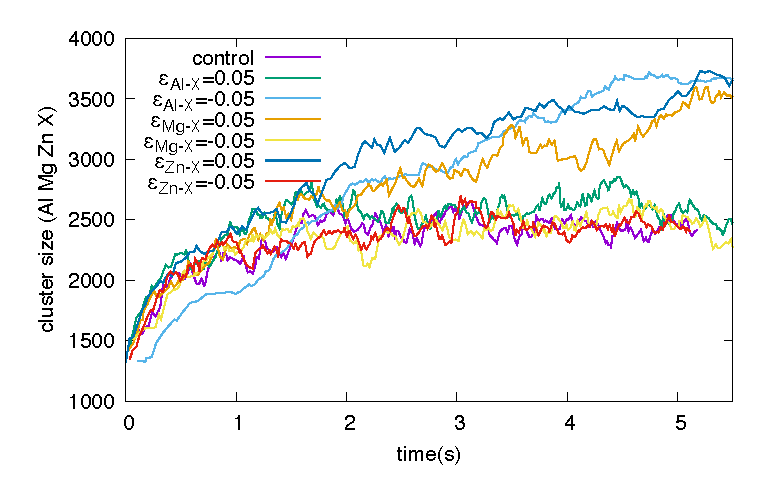
\includegraphics[width=0.8\linewidth]{Chap5/plots/size.eps}}
  \subfigure[Al Mg Zn]{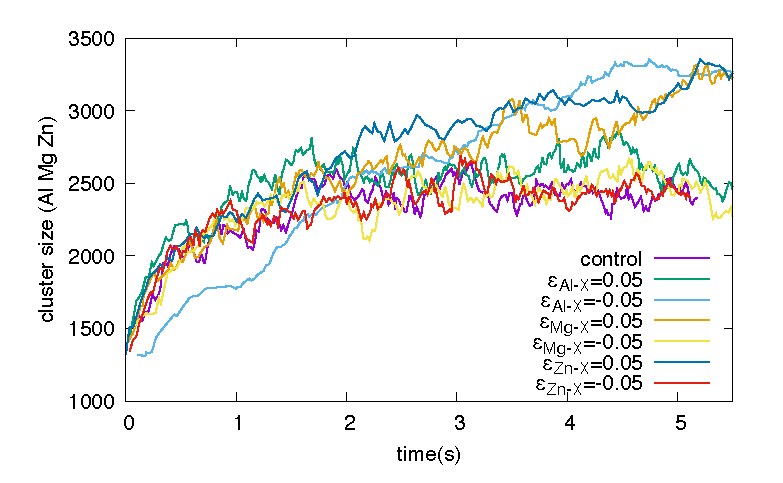
\includegraphics[width=0.8\linewidth]{Chap5/plots/size_noX.eps}}
\caption[Size changes of different clusters vs. time using $size_{critical}$ of 3 and $bond_{critical}$ of 3.]{Size changes of different clusters vs. time using $size_{critical}$ of 3 and $bond_{critical}$ of 3. Subplot. (a) is for all the atoms including pseudo atoms. (b) is for Al, Mg, and Zn only.}
\label{Chap:Al/Vac:fig:sens_cluster_size}
\end{figure}
\endgroup


\newpage
\begingroup
\begin{figure}[!ht]
  \centering
  \subfigure[cluster]{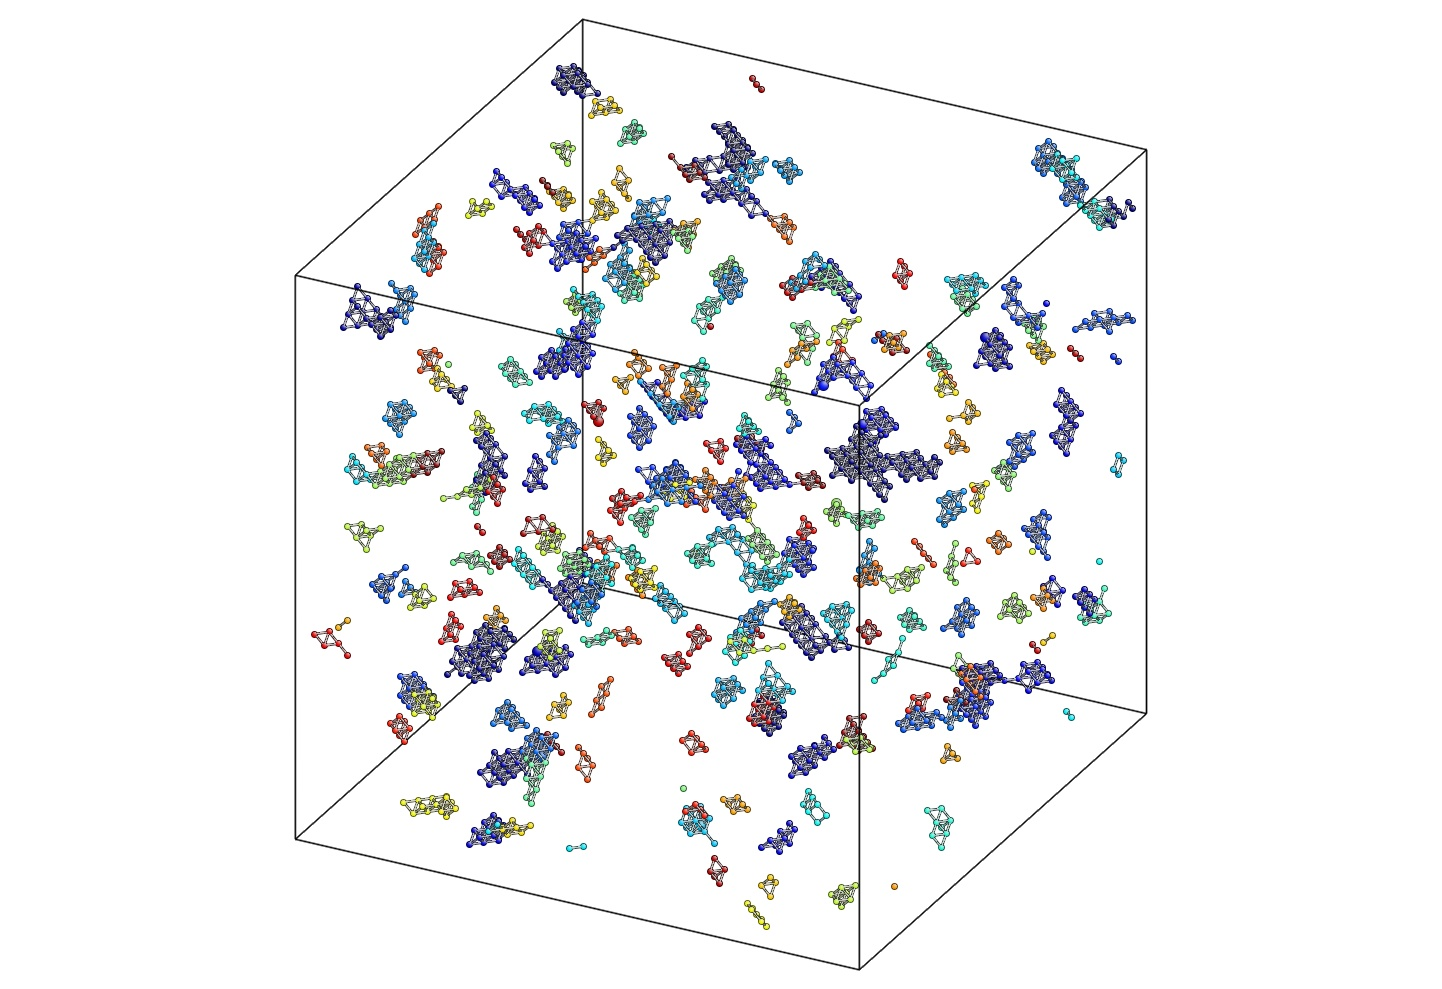
\includegraphics[width=0.8\linewidth]{Chap5/plots/cluster_id_jpg/00000.jpg}}
  \subfigure[species]{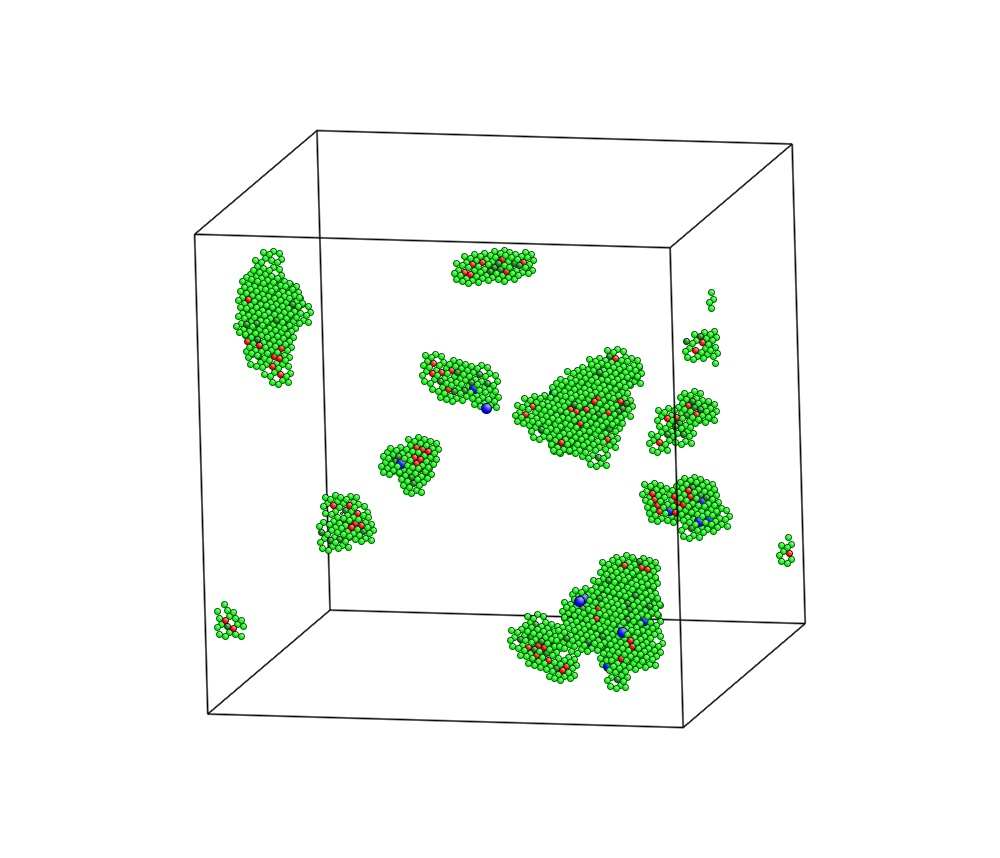
\includegraphics[width=0.8\linewidth]{Chap5/plots/element_jpg/00000.jpg}}
\caption[Atomistic pictures of 108,000 atoms for $\varepsilon_{Al-X}$ sensitivity test.]{Atomistic pictures of 108,000 atoms for control group, corresponding to setup \#0 in Table. \ref{Chap:Al/Vac:tab:pseudo1}. Subplot. (a) is colored by cluster size. The color mapping from dark blue to red is ranked by the cluster size in descending order. Subplot. (b) is colored by atom species. Light green, dark green, red, and blue atoms are Al, Mg, Zn, and pseudo atoms respectively.}
\label{Chap:Al/Vac:fig:sens_control}
\end{figure}
\endgroup


\newpage
\begingroup
\begin{figure}[!ht]
  \centering
  \subfigure[ratio of Al/(Mg+Zn)]{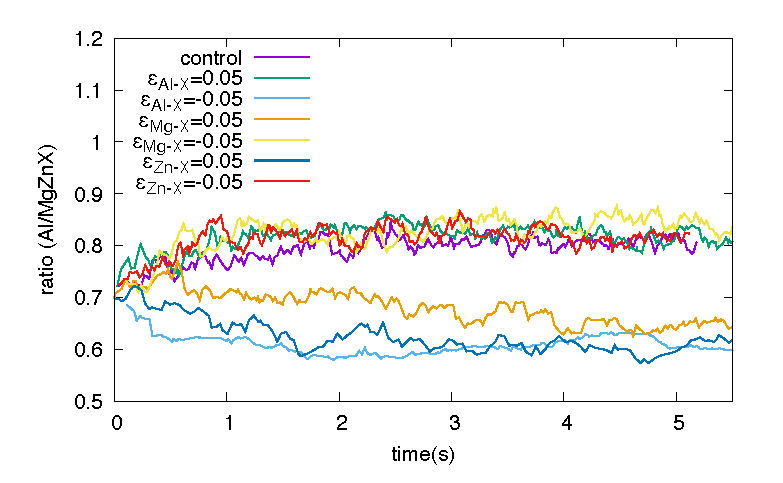
\includegraphics[width=0.8\linewidth]{Chap5/plots/ratio_Al-MgZnX.eps}}
  \subfigure[ratio of Mg/Zn]{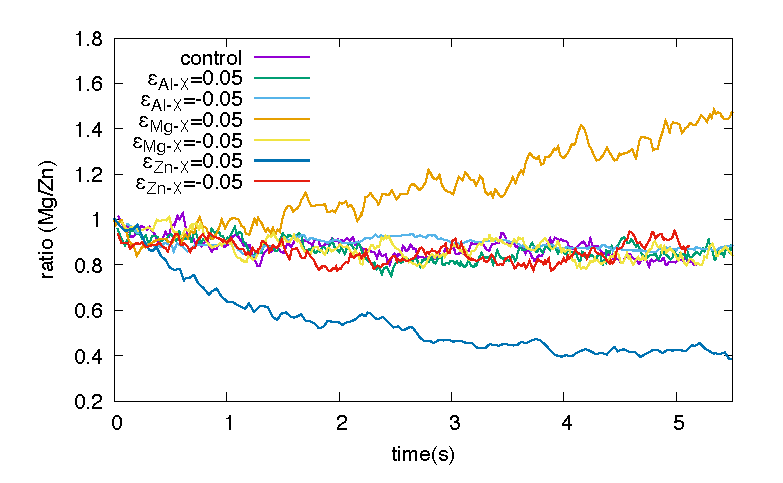
\includegraphics[width=0.8\linewidth]{Chap5/plots/ratio_Mg-Zn.eps}}
\caption[Ratio changes of different clusters vs. time using $size_{critical}$ of 3 and $bond_{critical}$ of 3.]{Ratio changes of different clusters vs. time using $size_{critical}$ of 3 and $bond_{critical}$ of 3. Subplot. (a) is for the ratio between all the Al atoms and the sum of Mg and Zn atoms in the clusters. (b) is for Mg and Zn ratio in the clusters.}
\label{Chap:Al/Vac:fig:sens_cluster_ratio}
\end{figure}
\endgroup


\newpage
\begingroup
\begin{figure}[!ht]
  \centering
  \subfigure[$\varepsilon_{Al-X} = 0.05$ cluster]{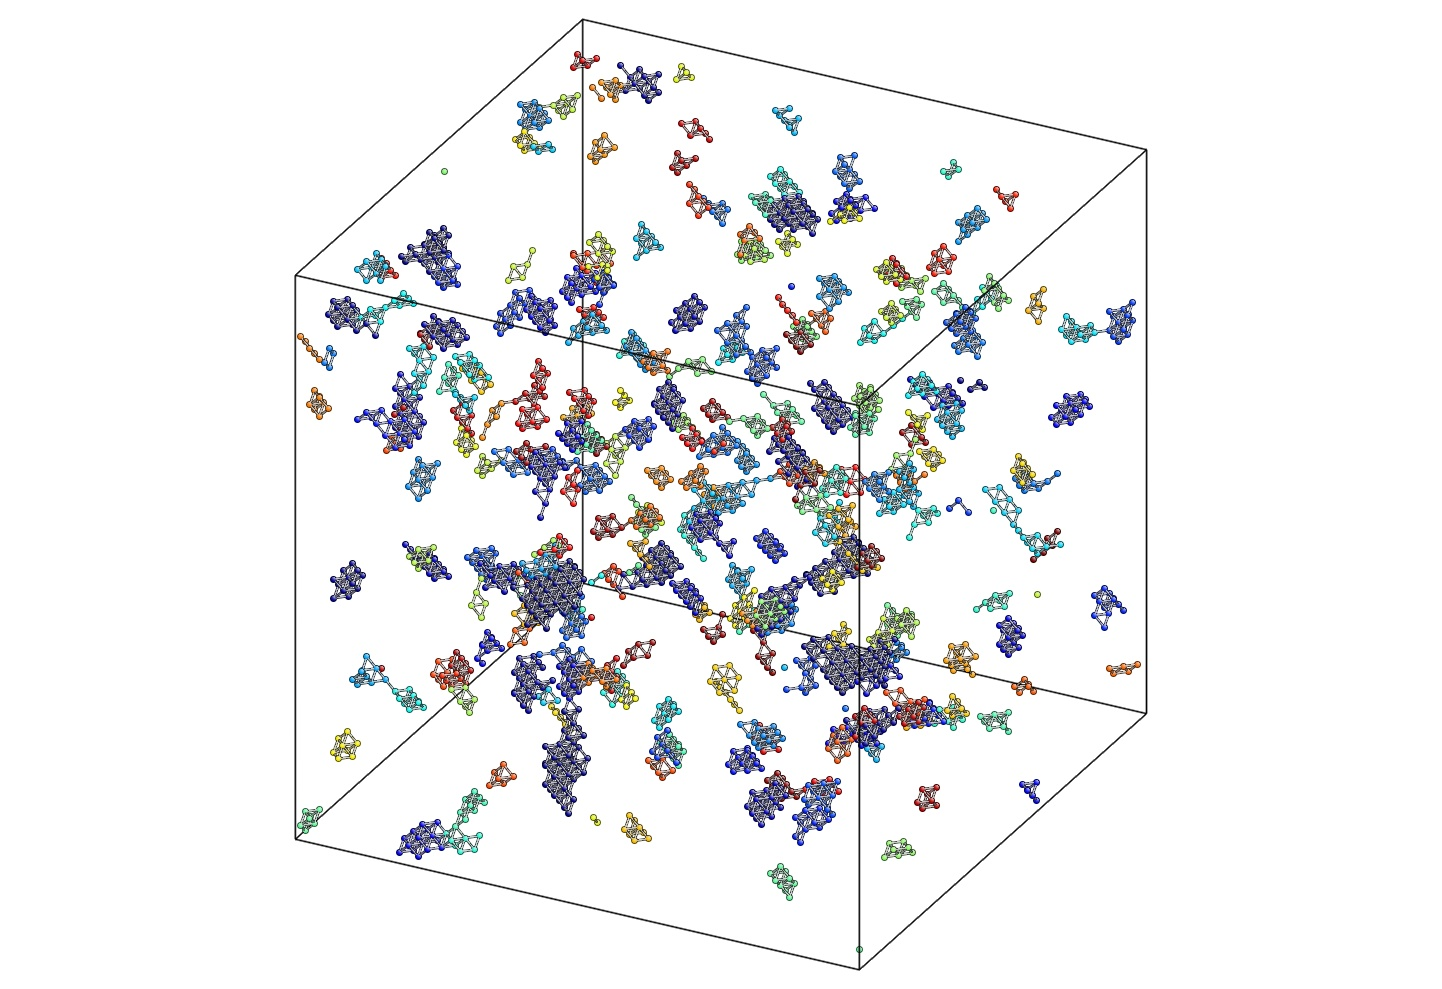
\includegraphics[width=0.49\linewidth]{Chap5/plots/cluster_id_jpg/00001.jpg}}
%   \subfigure[controlcluster]{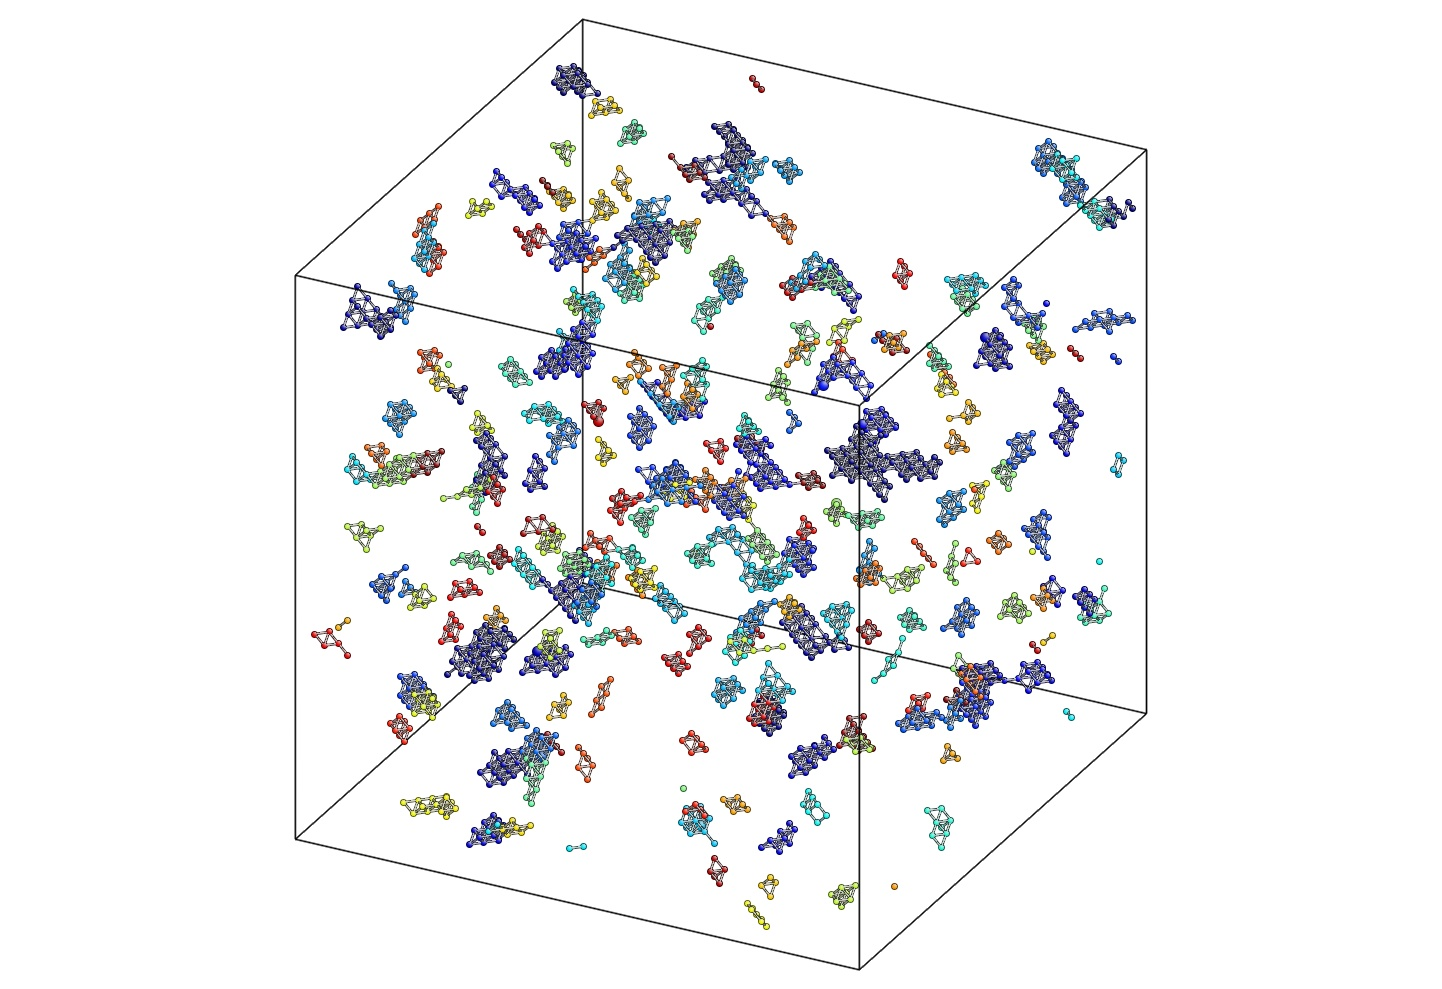
\includegraphics[width=0.49\linewidth]{Chap5/plots/cluster_id_jpg/00000.jpg}}
  \subfigure[$\varepsilon_{Al-X} = -0.05$ cluster]{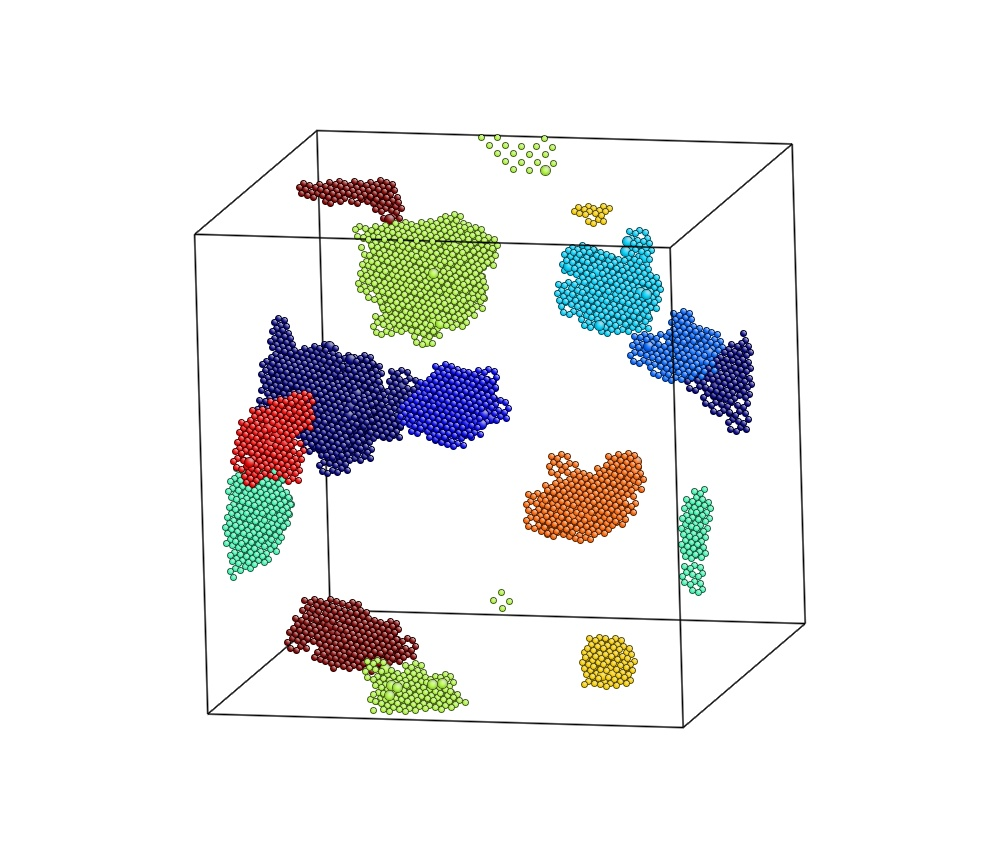
\includegraphics[width=0.49\linewidth]{Chap5/plots/cluster_id_jpg/00002.jpg}}
  \subfigure[$\varepsilon_{Al-X} = 0.05$ species]{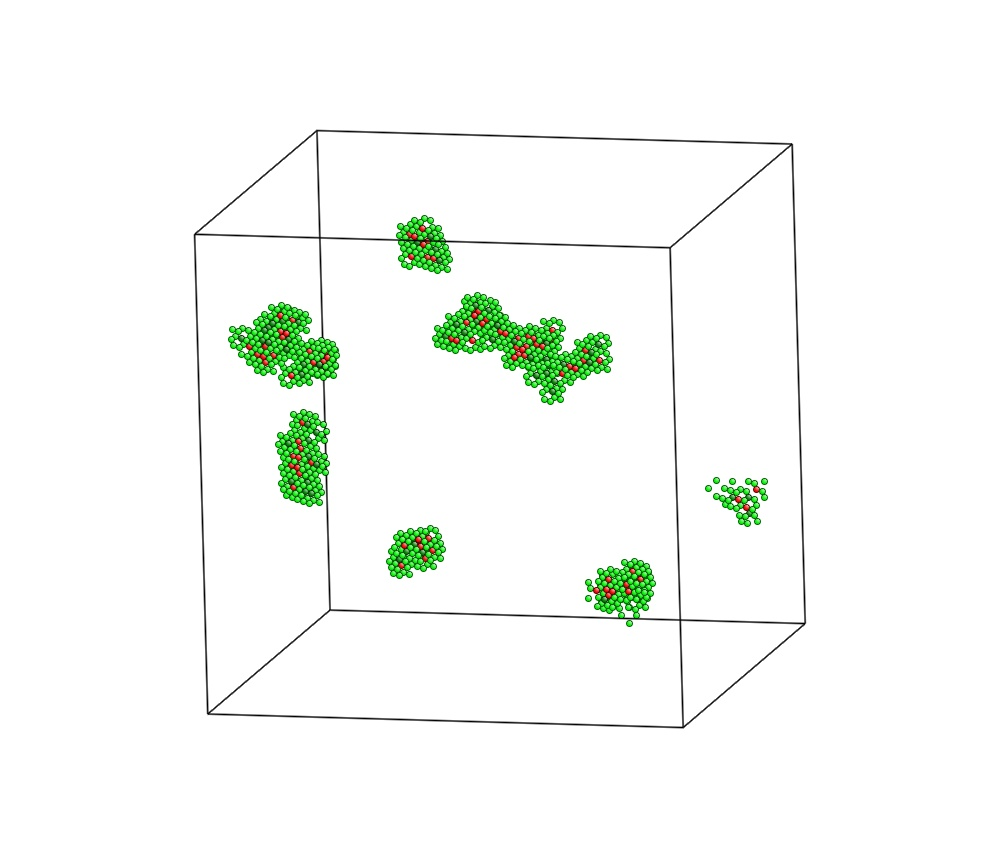
\includegraphics[width=0.49\linewidth]{Chap5/plots/element_jpg/00001.jpg}}
%   \subfigure[control species]{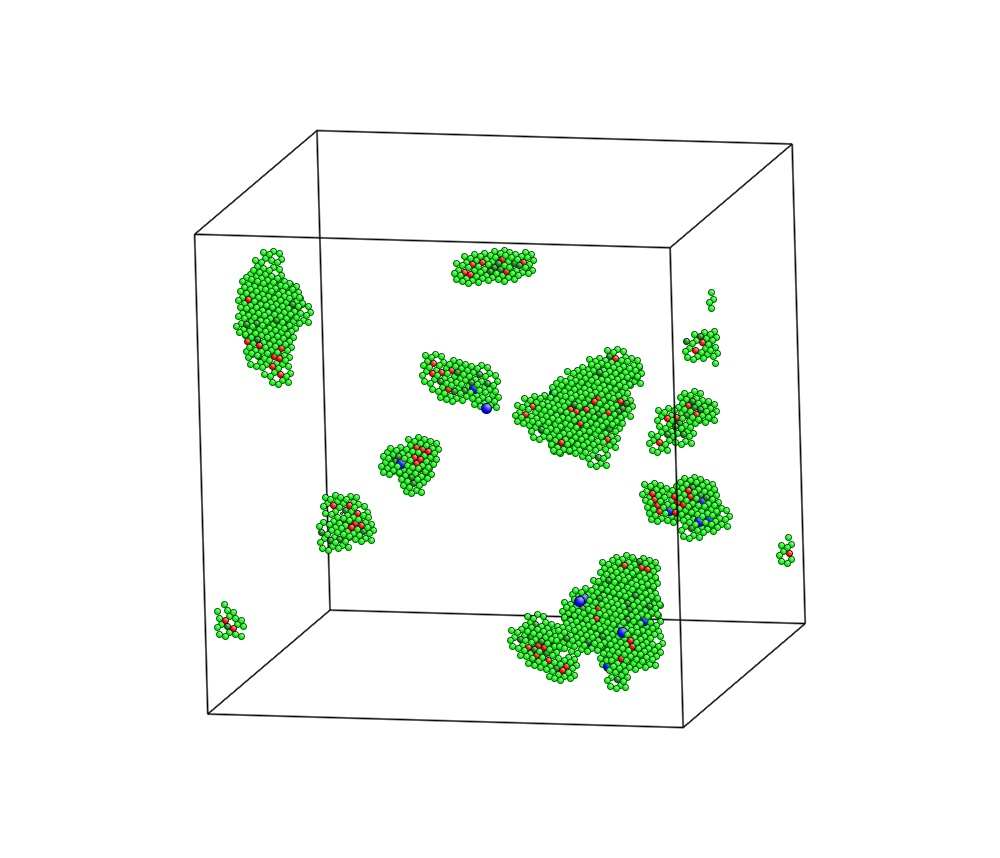
\includegraphics[width=0.49\linewidth]{Chap5/plots/element_jpg/00000.jpg}}
  \subfigure[$\varepsilon_{Al-X} = -0.05$ species]{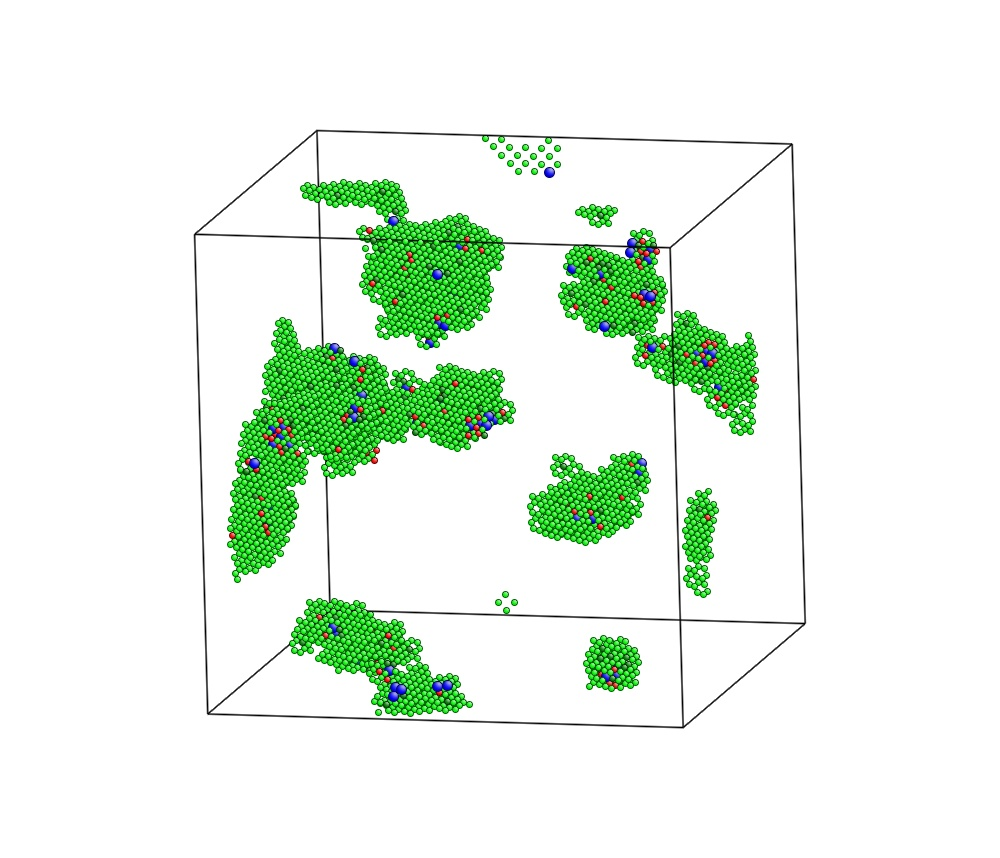
\includegraphics[width=0.49\linewidth]{Chap5/plots/element_jpg/00002.jpg}}
% \caption[Atomistic pictures of 108,000 atoms for $\varepsilon_{Al-X}$ sensitivity test.]{Atomistic pictures of 108,000 atoms for $\varepsilon_{Al-X}$ sensitivity test. (a), (d) : $\varepsilon_{Al-X} = 0.05$, which is setup \#1 in Table. \ref{Chap:Al/Vac:tab:pseudo1}. (b), (e) : setup \#0 in Table. \ref{Chap:Al/Vac:tab:pseudo1}. (c), (f) : $\varepsilon_{Al-X} = -0.05$, which is setup \#2 in Table. \ref{Chap:Al/Vac:tab:pseudo1}. (a), (b), and (c) are colored by cluster size. The color mapping from dark blue to red is ranked by the cluster size in descending order. (d), (e), and (f) are colored by atom species.  Light green, dark green, red, and blue atoms are Al, Mg, Zn, and pseudo atoms respectively.}
\caption[Atomistic pictures of 108,000 atoms for $\varepsilon_{Al-X}$ sensitivity test.]{Atomistic pictures of 108,000 atoms for $\varepsilon_{Al-X}$ sensitivity test. (a), (c) : $\varepsilon_{Al-X} = 0.05$, which is setup \#1 in Table. \ref{Chap:Al/Vac:tab:pseudo1}. (b), (d) : $\varepsilon_{Al-X} = -0.05$, which is setup \#2 in Table. \ref{Chap:Al/Vac:tab:pseudo1}. (a) and (c) are colored by cluster size. The color mapping from dark blue to red is ranked by the cluster size in descending order. (b) and (d) are colored by atom species. Light green, dark green, red, and blue atoms are Al, Mg, Zn, and pseudo atoms respectively.}
\label{Chap:Al/Vac:fig:sens_Al}
\end{figure}
\endgroup


\newpage
\begingroup
\begin{figure}[!ht]
  \centering
  \subfigure[$\varepsilon_{Mg-X} = 0.05$ cluster]{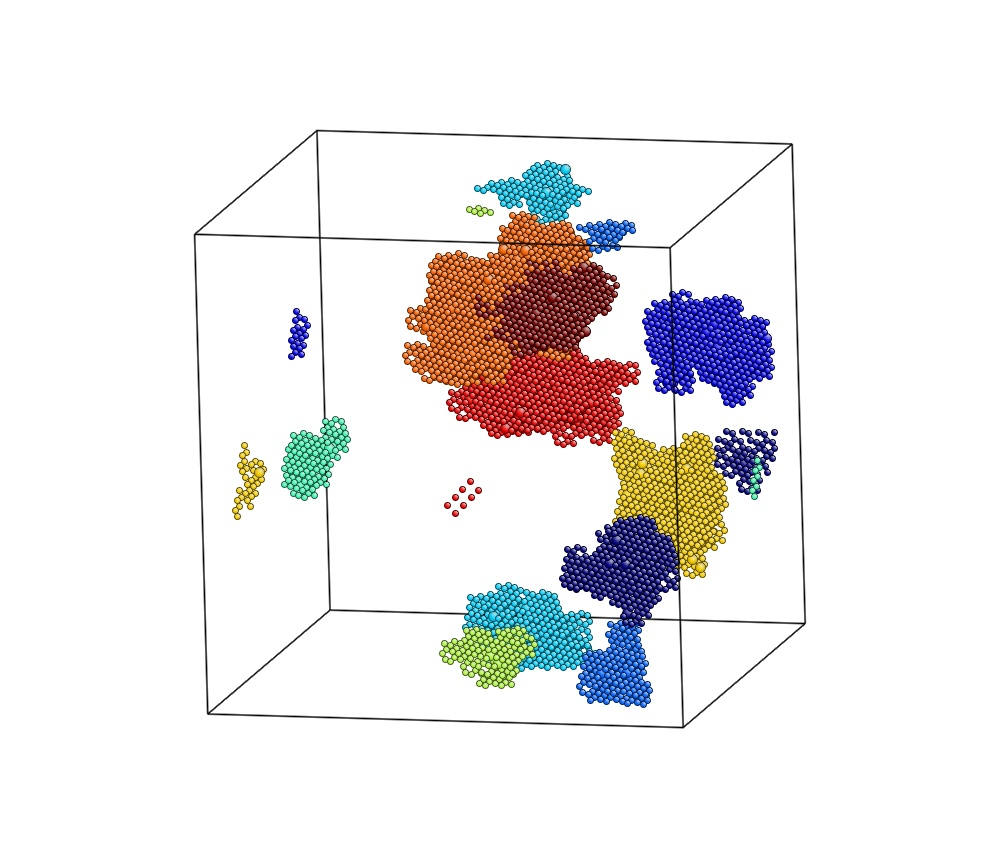
\includegraphics[width=0.49\linewidth]{Chap5/plots/cluster_id_jpg/00003.jpg}}
%   \subfigure[control]{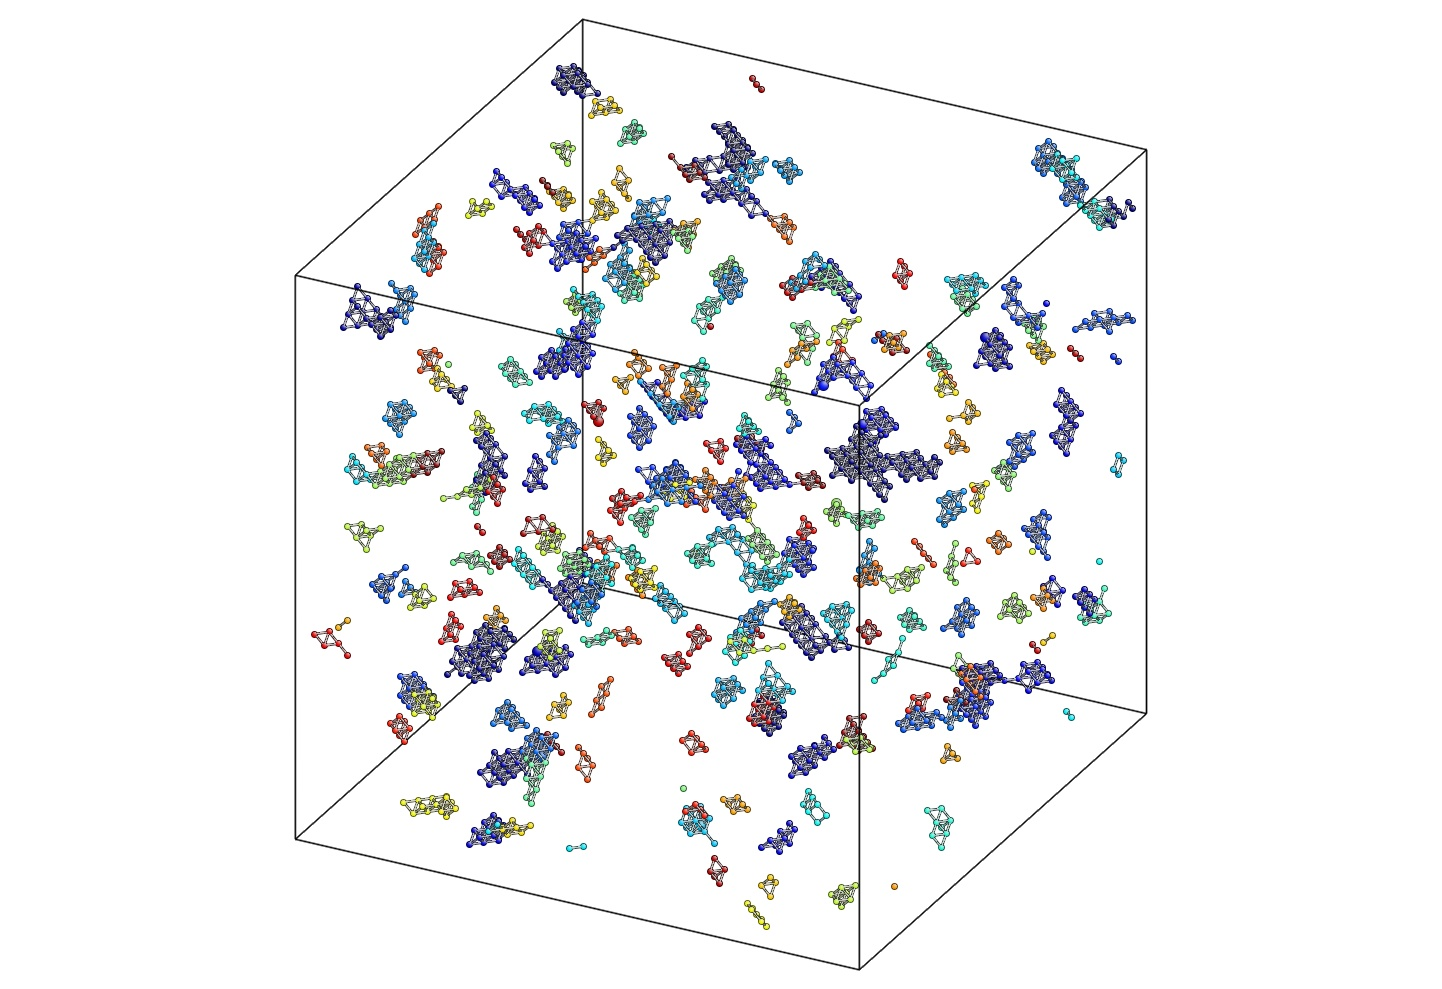
\includegraphics[width=0.32\linewidth]{Chap5/plots/cluster_id_jpg/00000.jpg}}
  \subfigure[$\varepsilon_{Mg-X} = -0.05$ cluster]{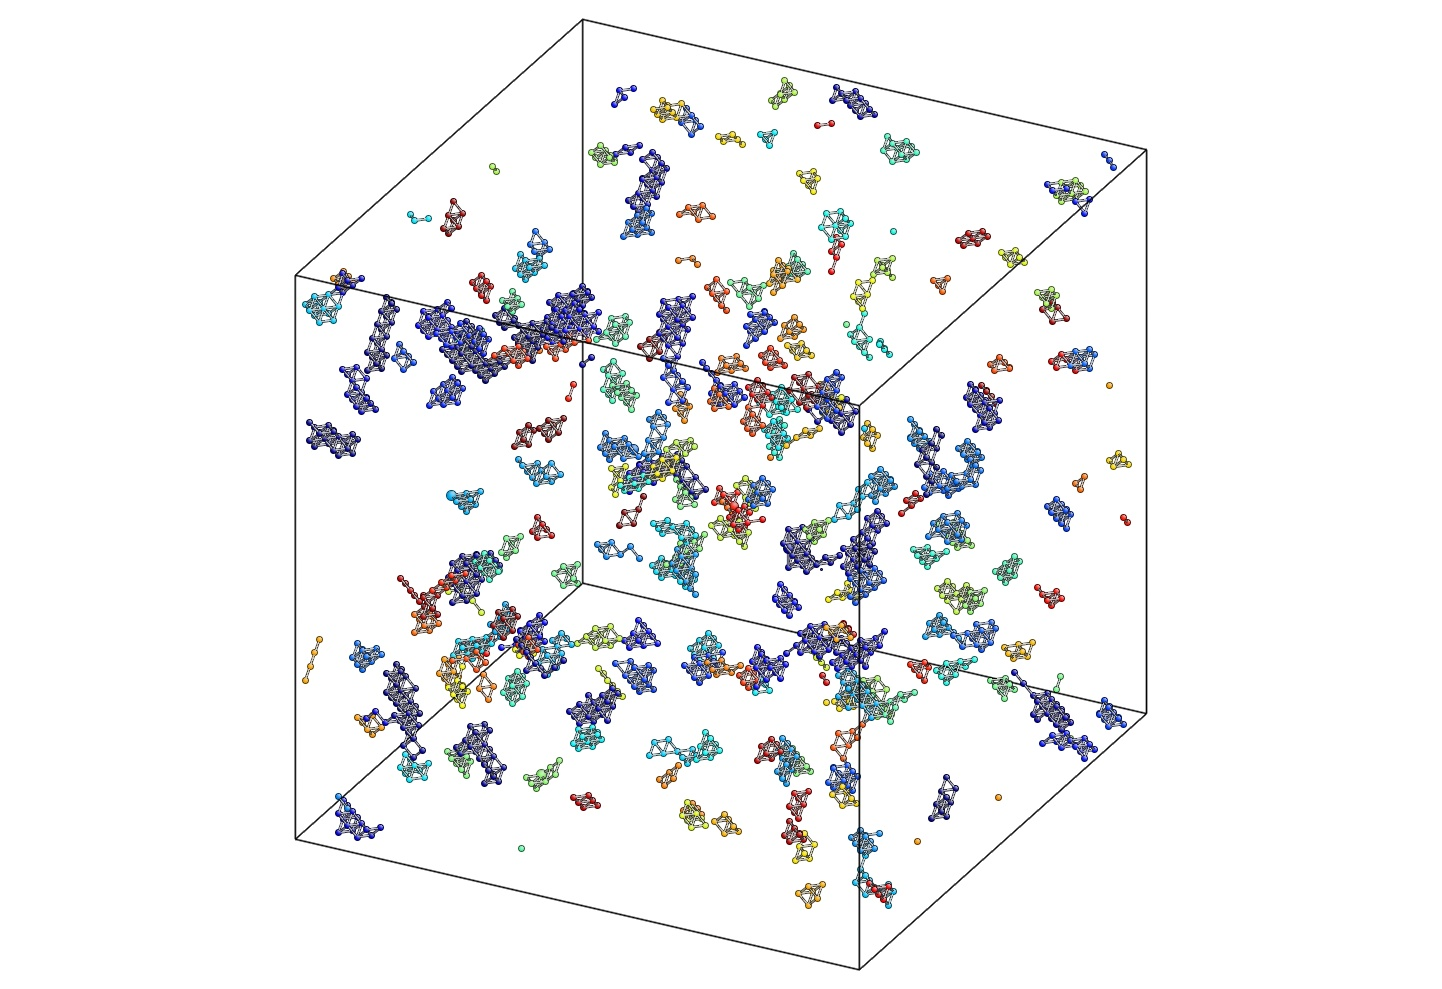
\includegraphics[width=0.49\linewidth]{Chap5/plots/cluster_id_jpg/00004.jpg}} \\
  \subfigure[$\varepsilon_{Mg-X} = 0.05$ species]{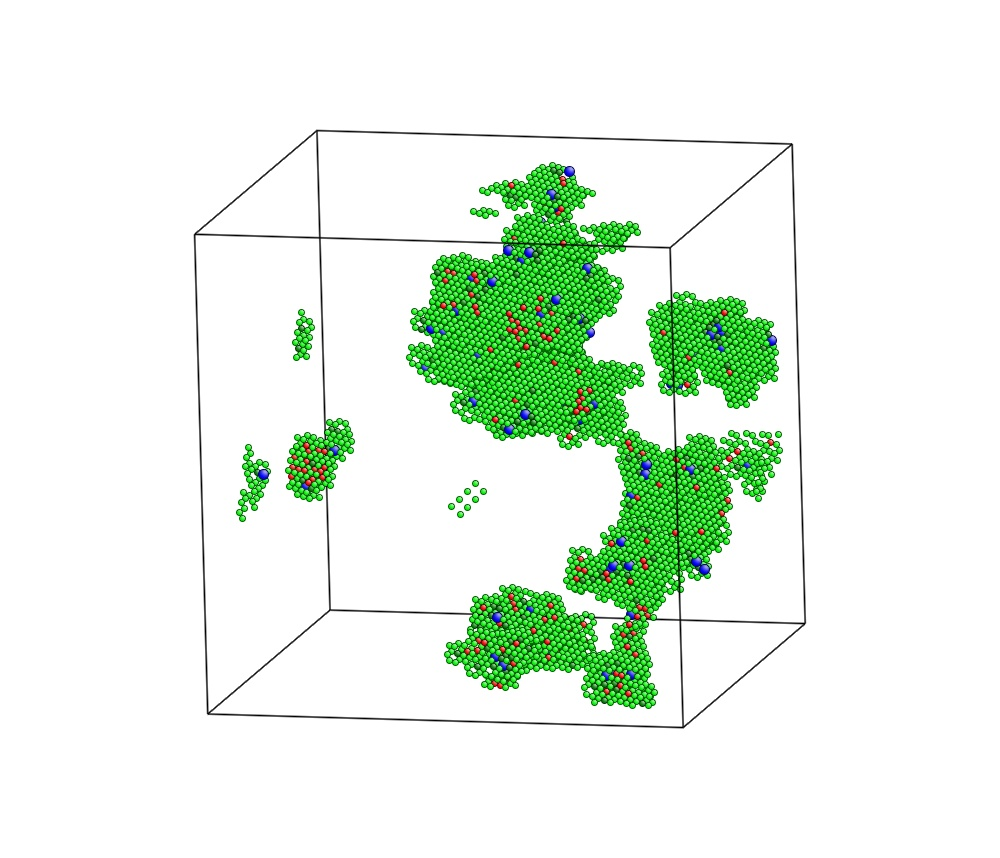
\includegraphics[width=0.49\linewidth]{Chap5/plots/element_jpg/00003.jpg}}
%   \subfigure[control]{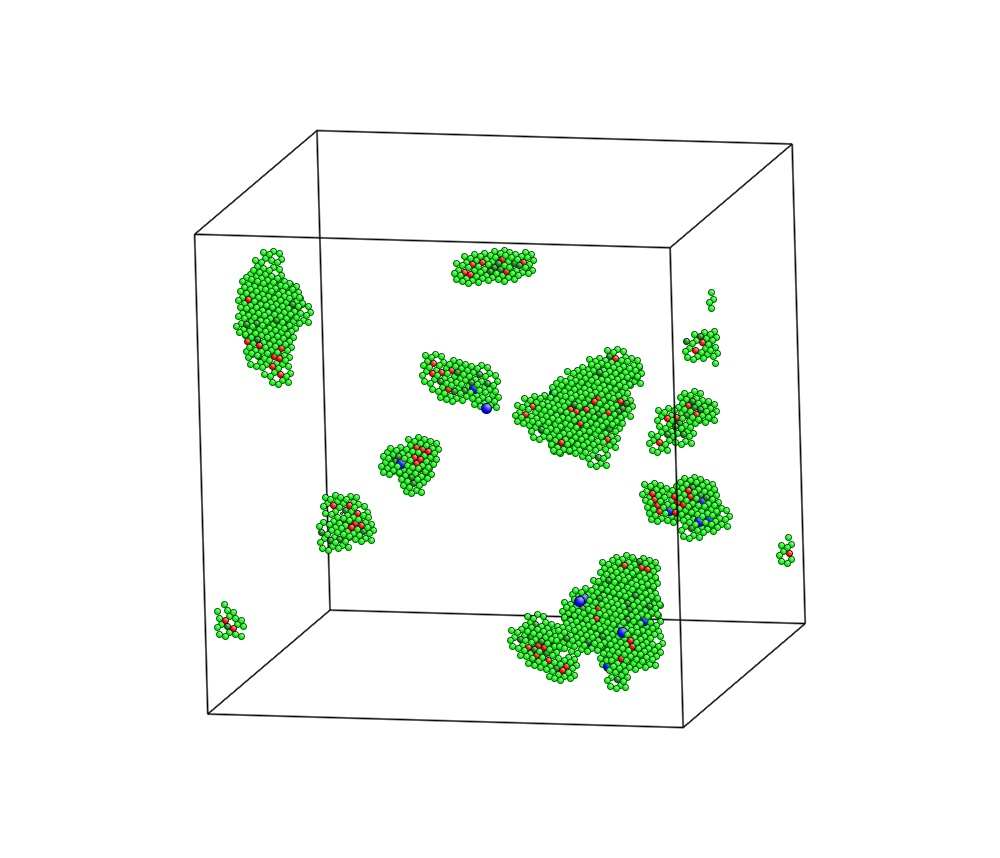
\includegraphics[width=0.32\linewidth]{Chap5/plots/element_jpg/00000.jpg}}
  \subfigure[$\varepsilon_{Mg-X} = -0.05$ species]{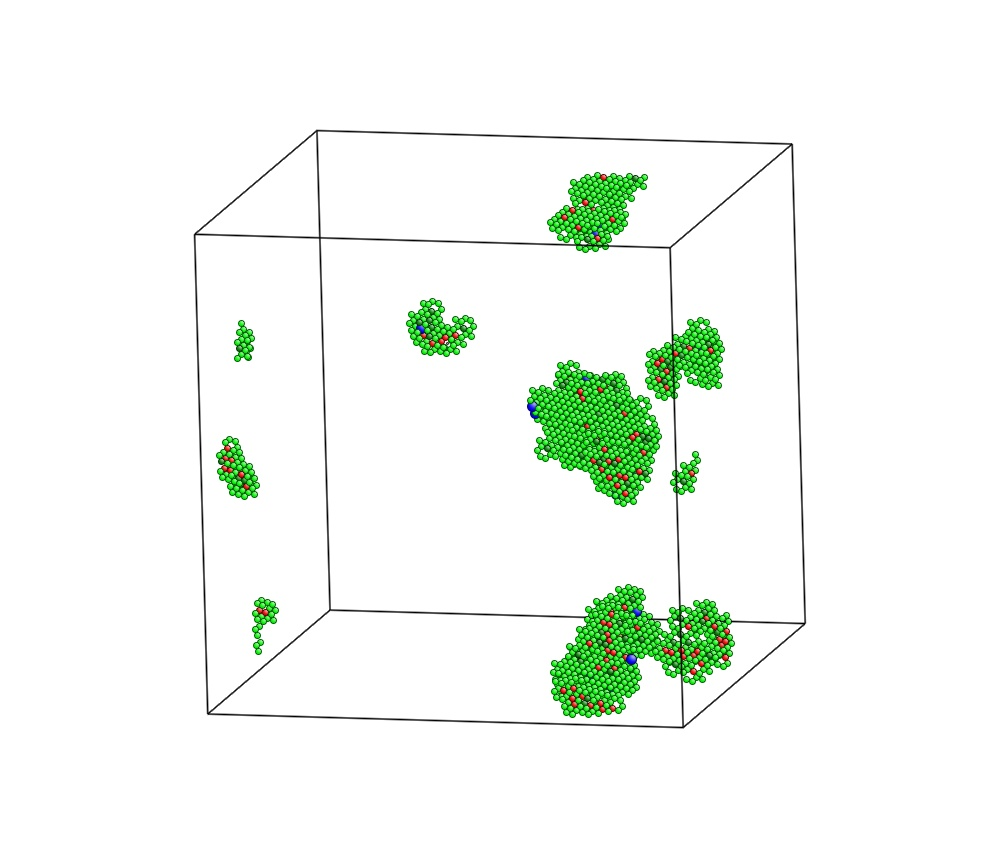
\includegraphics[width=0.49\linewidth]{Chap5/plots/element_jpg/00004.jpg}}
% \caption[Atomistic pictures of 108,000 atoms for $\varepsilon_{Mg-X}$ sensitivity test.]{Atomistic pictures of 108,000 atoms for $\varepsilon_{Mg-X}$ sensitivity test. (a), (d) : $\varepsilon_{Mg-X} = 0.05$, which is setup \#3 in Table. \ref{Chap:Al/Vac:tab:pseudo1}. (b), (e) : setup \#0 in Table. \ref{Chap:Al/Vac:tab:pseudo1}. (c), (f) : $\varepsilon_{Mg-X} = -0.05$, which is setup \#4 in Table. \ref{Chap:Al/Vac:tab:pseudo1}. (a), (b), and (c) are colored by cluster size. The color mapping from dark blue to red is ranked by the cluster size in descending order. (d), (e), and (f) are colored by atom species.  Light green, dark green, red, and blue atoms are Al, Mg, Zn, and pseudo atoms respectively.}
\caption[Atomistic pictures of 108,000 atoms for $\varepsilon_{Mg-X}$ sensitivity test.]{Atomistic pictures of 108,000 atoms for $\varepsilon_{Mg-X}$ sensitivity test. (a), (c) : $\varepsilon_{Mg-X} = 0.05$, which is setup \#3 in Table. \ref{Chap:Al/Vac:tab:pseudo1}. (b), (d) : $\varepsilon_{Mg-X} = -0.05$, which is setup \#4 in Table. \ref{Chap:Al/Vac:tab:pseudo1}. (a) and (c) are colored by cluster size. The color mapping from dark blue to red is ranked by the cluster size in descending order. (b) and (d) are colored by atom species. Light green, dark green, red, and blue atoms are Al, Mg, Zn, and pseudo atoms respectively.}
\label{Chap:Al/Vac:fig:sens_Mg}
\end{figure}
\endgroup

\newpage
\begingroup
\begin{figure}[!ht]
  \centering
  \subfigure[$\varepsilon_{Zn-X} = 0.05$ cluster]{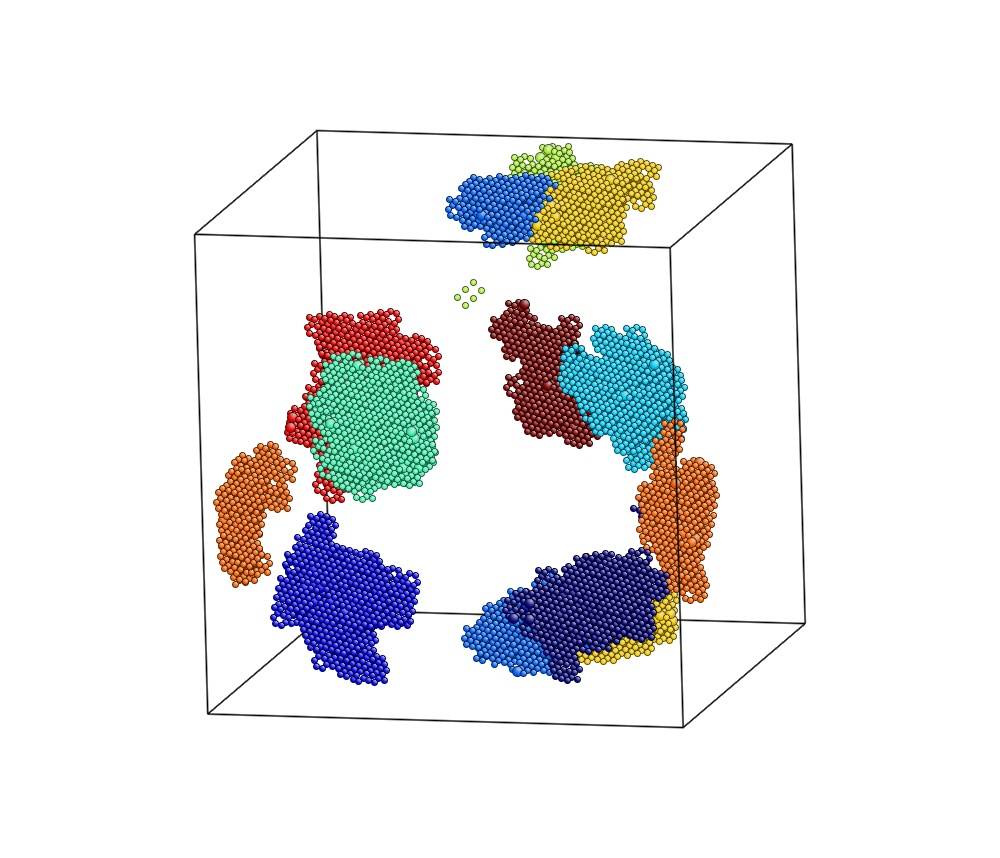
\includegraphics[width=0.49\linewidth]{Chap5/plots/cluster_id_jpg/00005.jpg}}
%   \subfigure[control]{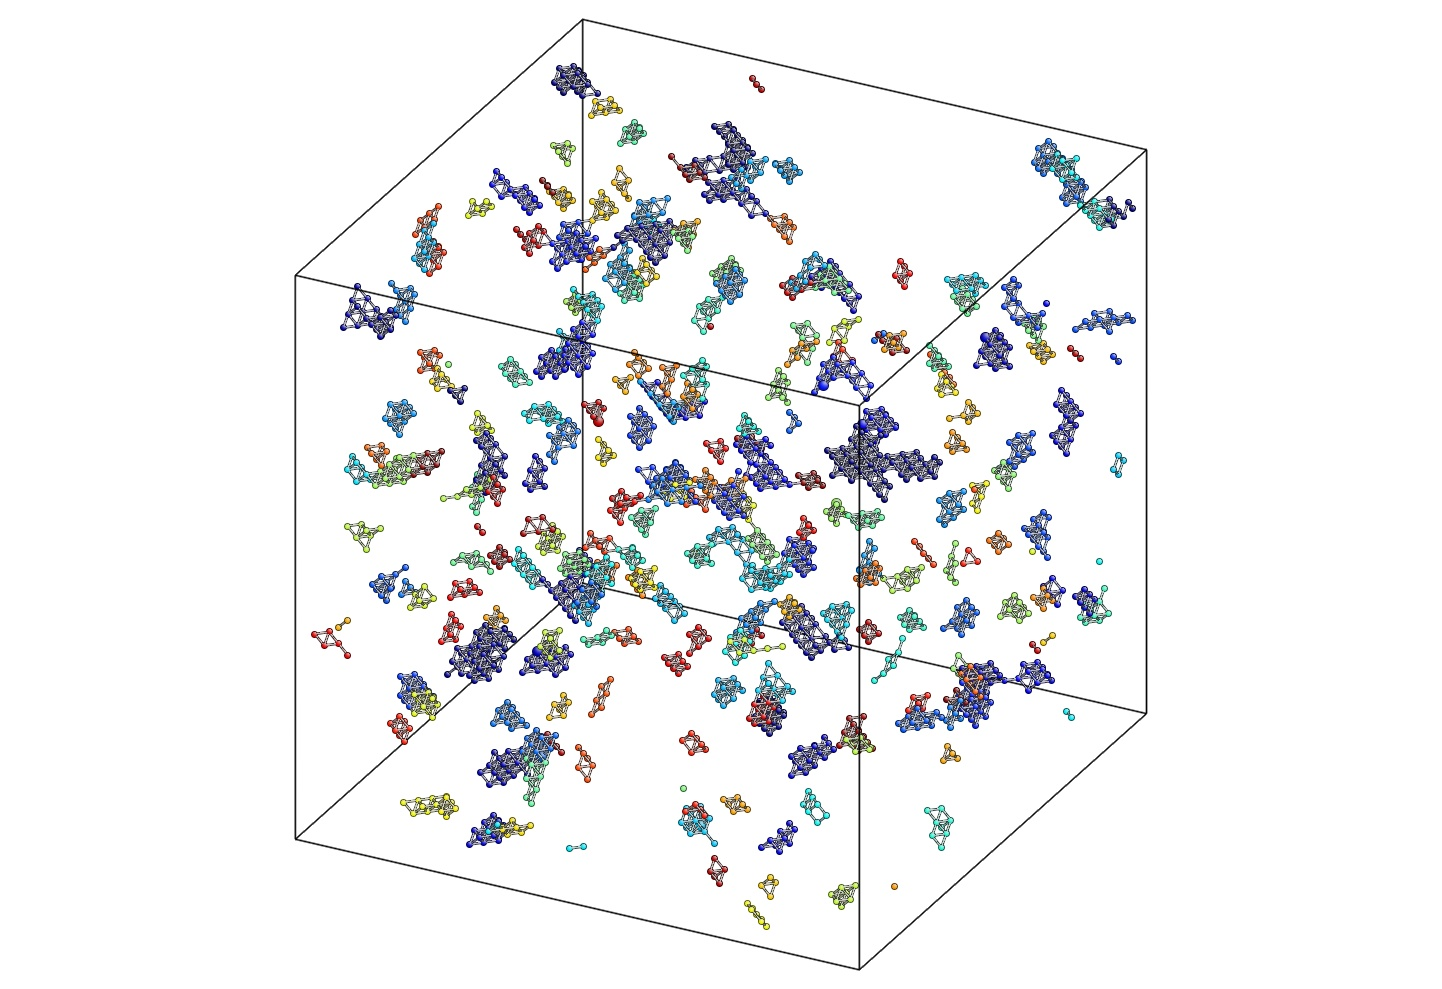
\includegraphics[width=0.32\linewidth]{Chap5/plots/cluster_id_jpg/00000.jpg}}
  \subfigure[$\varepsilon_{Zn-X} = -0.05$ cluster]{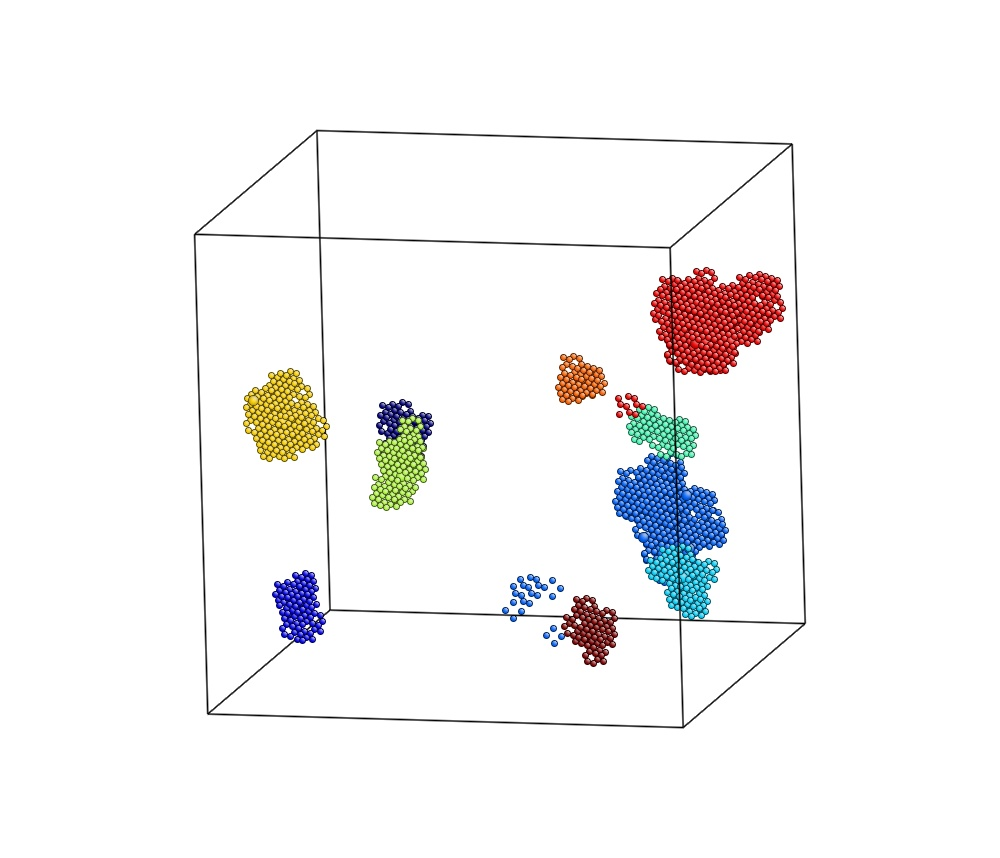
\includegraphics[width=0.49\linewidth]{Chap5/plots/cluster_id_jpg/00006.jpg}} \\
  \subfigure[$\varepsilon_{Zn-X} = 0.05$ species]{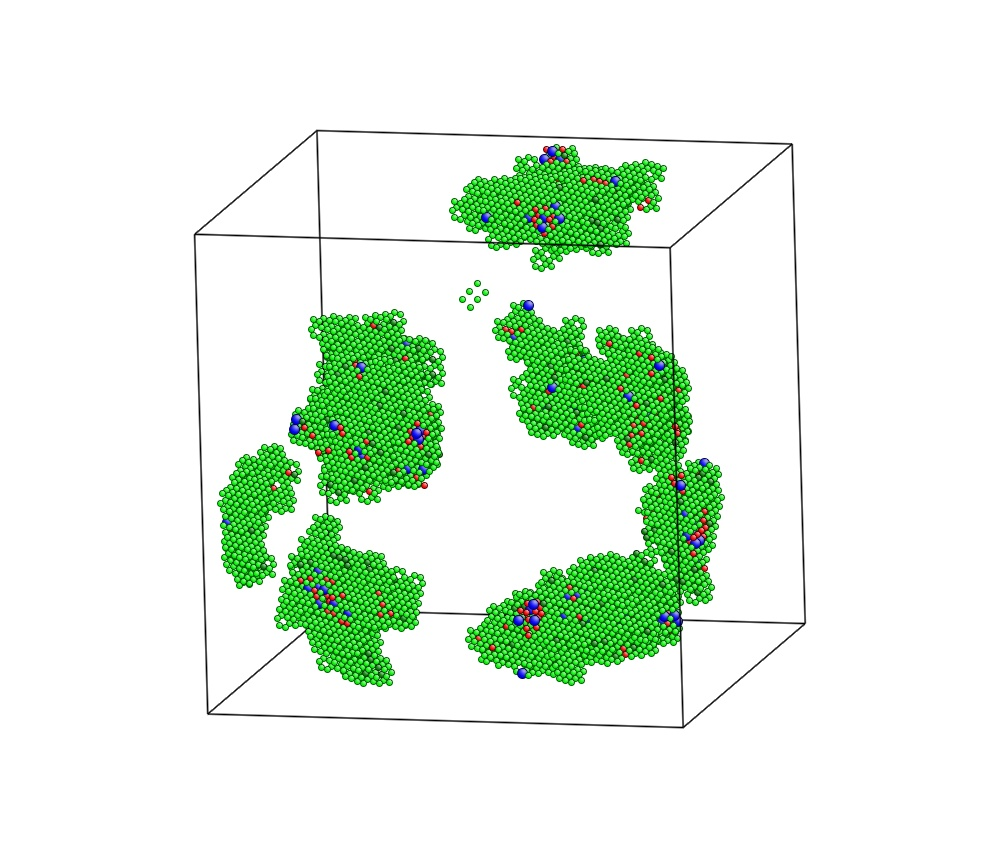
\includegraphics[width=0.49\linewidth]{Chap5/plots/element_jpg/00005.jpg}}
%   \subfigure[control]{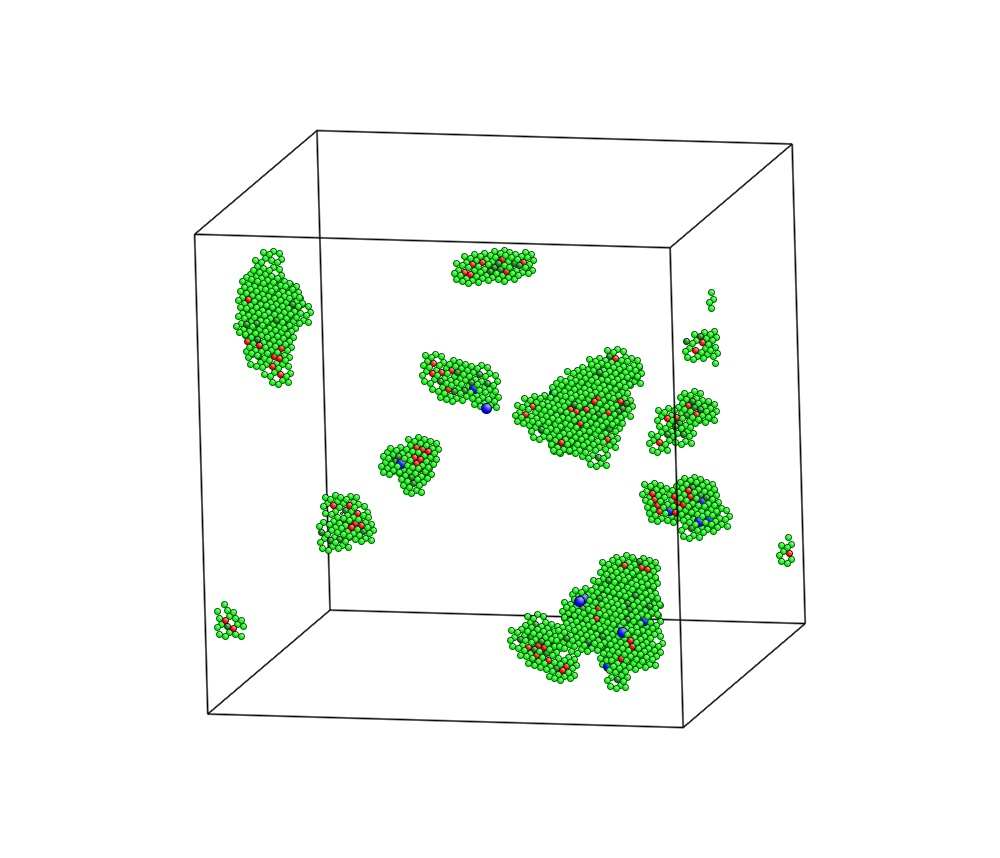
\includegraphics[width=0.32\linewidth]{Chap5/plots/element_jpg/00000.jpg}}
  \subfigure[$\varepsilon_{Zn-X} = -0.05$ species]{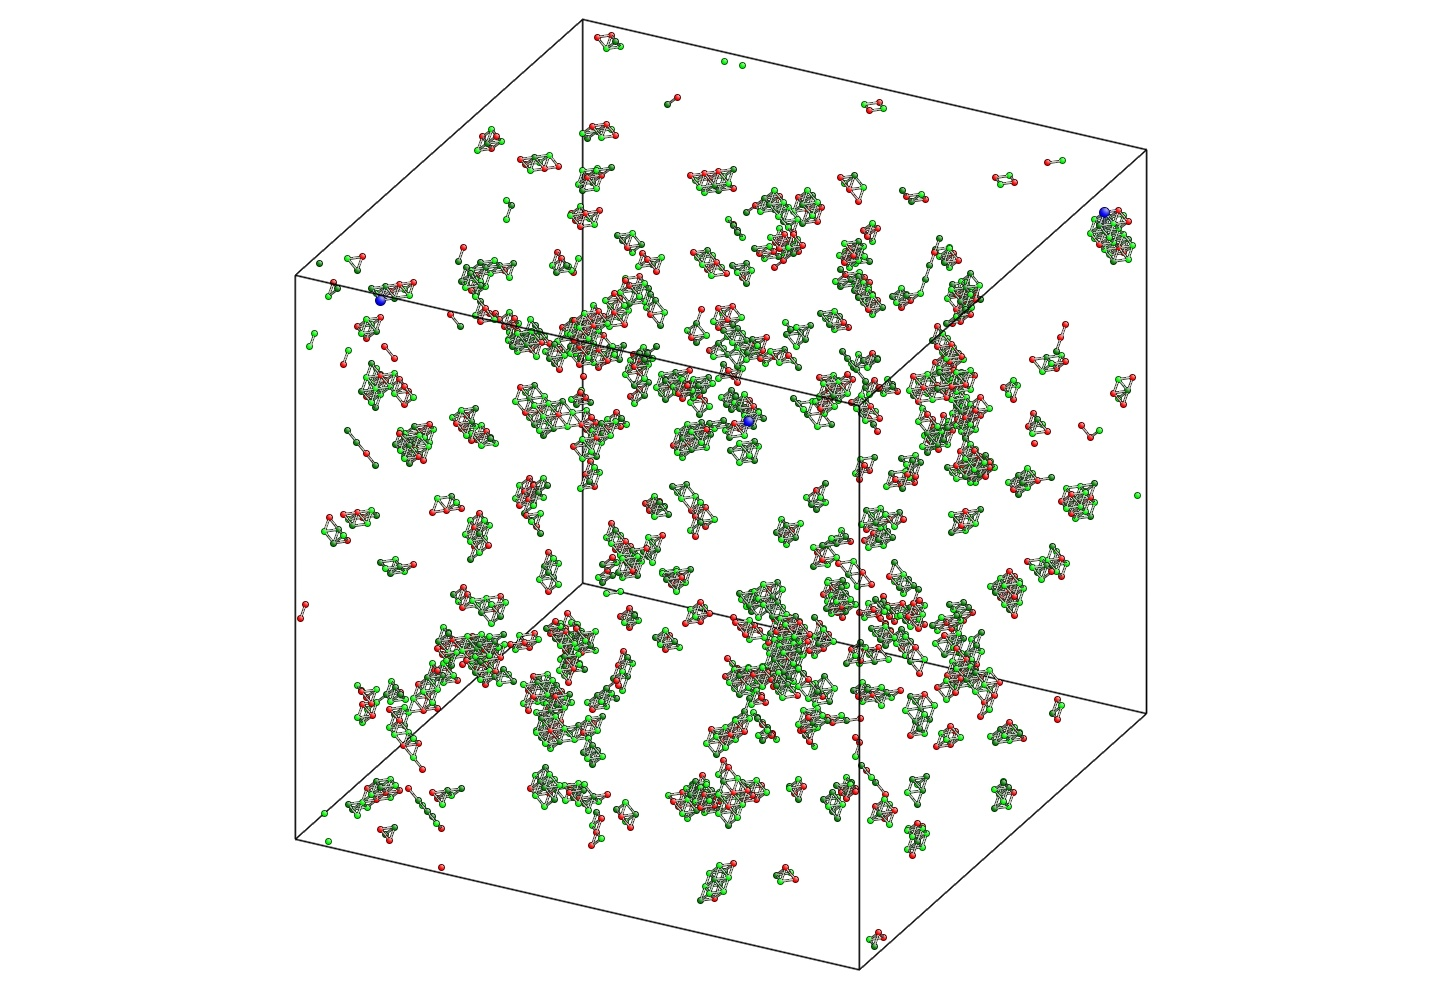
\includegraphics[width=0.49\linewidth]{Chap5/plots/element_jpg/00006.jpg}}
% \caption[Atomistic pictures of 108,000 atoms for $\varepsilon_{Zn-X}$ sensitivity test.]{Atomistic pictures of 108,000 atoms for $\varepsilon_{Zn-X}$ sensitivity test. (a), (d) : $\varepsilon_{Zn-X} = 0.05$, which is setup \#5 in Table. \ref{Chap:Al/Vac:tab:pseudo1}. (b), (e) : setup \#0 in Table. \ref{Chap:Al/Vac:tab:pseudo1}. (c), (f) : $\varepsilon_{Zn-X} = -0.05$, which is setup \#6 in Table. \ref{Chap:Al/Vac:tab:pseudo1}. (a), (b), and (c) are colored by cluster size. The color mapping from dark blue to red is ranked by the cluster size in descending order. (d), (e), and (f) are colored by atom species.  Light green, dark green, red, and blue atoms are Al, Mg, Zn, and pseudo atoms respectively.}
\caption[Atomistic pictures of 108,000 atoms for $\varepsilon_{Zn-X}$ sensitivity test.]{Atomistic pictures of 108,000 atoms for $\varepsilon_{Zn-X}$ sensitivity test. (a), (c) : $\varepsilon_{Zn-X} = 0.05$, which is setup \#5 in Table. \ref{Chap:Al/Vac:tab:pseudo1}. (b), (d) : $\varepsilon_{Zn-X} = -0.05$, which is setup \#6 in Table. \ref{Chap:Al/Vac:tab:pseudo1}. (a) and (c) are colored by cluster size. The color mapping from dark blue to red is ranked by the cluster size in descending order. (b) and (d) are colored by atom species. Light green, dark green, red, and blue atoms are Al, Mg, Zn, and pseudo atoms respectively.}
\label{Chap:Al/Vac:fig:sens_Zn}
\end{figure}
\endgroup
\section{Conclusion}
\label{Chap:Al/Vac:section:Conc}


In this chapter, we first demonstrated that the \acf{BEP} relationship fails to provide quantitatively accurate diffusion barriers for multi-component alloys. Then we developed a \ac{NN} model to predict diffusion barriers using thousands of \ac{DFT} calculated barriers. And a \ac{kMC} method based on this \ac{NN} model is used to study the early transition behavior from a supersaturated solid solution to \ac{GP} zone of Al 7000 series alloys. A local super-basin method together with \ac{LRU} cache is also implemented to accelerate \ac{kMC} simulations. Following our general strategy to add a trace amount of element, we studied the effect of adding pseudo-atoms with different ability to change vacancy diffusion barriers. At last, we compared current methods to evaluate the strengthening effect of precipitates and proposed potential machine learning methods based on cluster geometry and chemical information. Quantitative analysis methods to describe the chemical and structural properties of clusters were developed, which could be used as inputs to predict precipitate strengthening effects. In the future, the output parameters and cluster atomic structures from this simulation will be used to predict the hardness at different nucleation stages.


\newpage
\begingroup
\begin{figure}[!ht]
  \centering
  \subfigure[$\varepsilon_{Mg-X} = 0.05$, cluster]{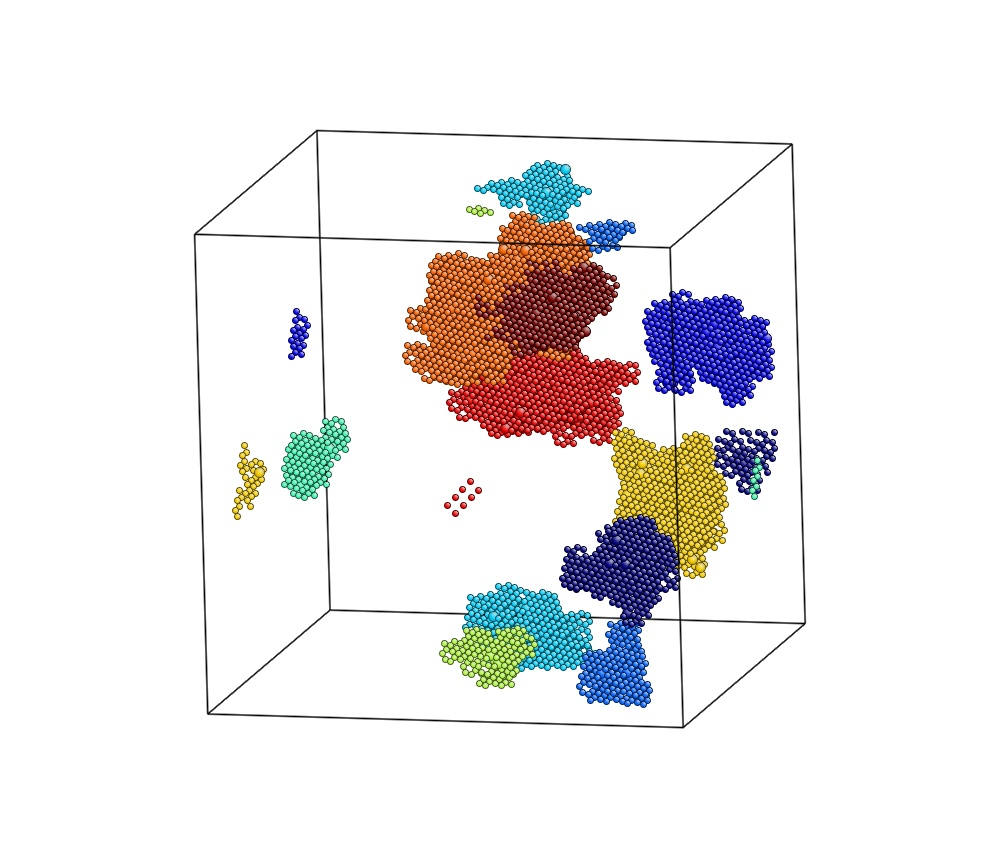
\includegraphics[width=0.49\linewidth]{Chap5/plots/cluster_id_jpg/00003.jpg}}
%   \subfigure[control]{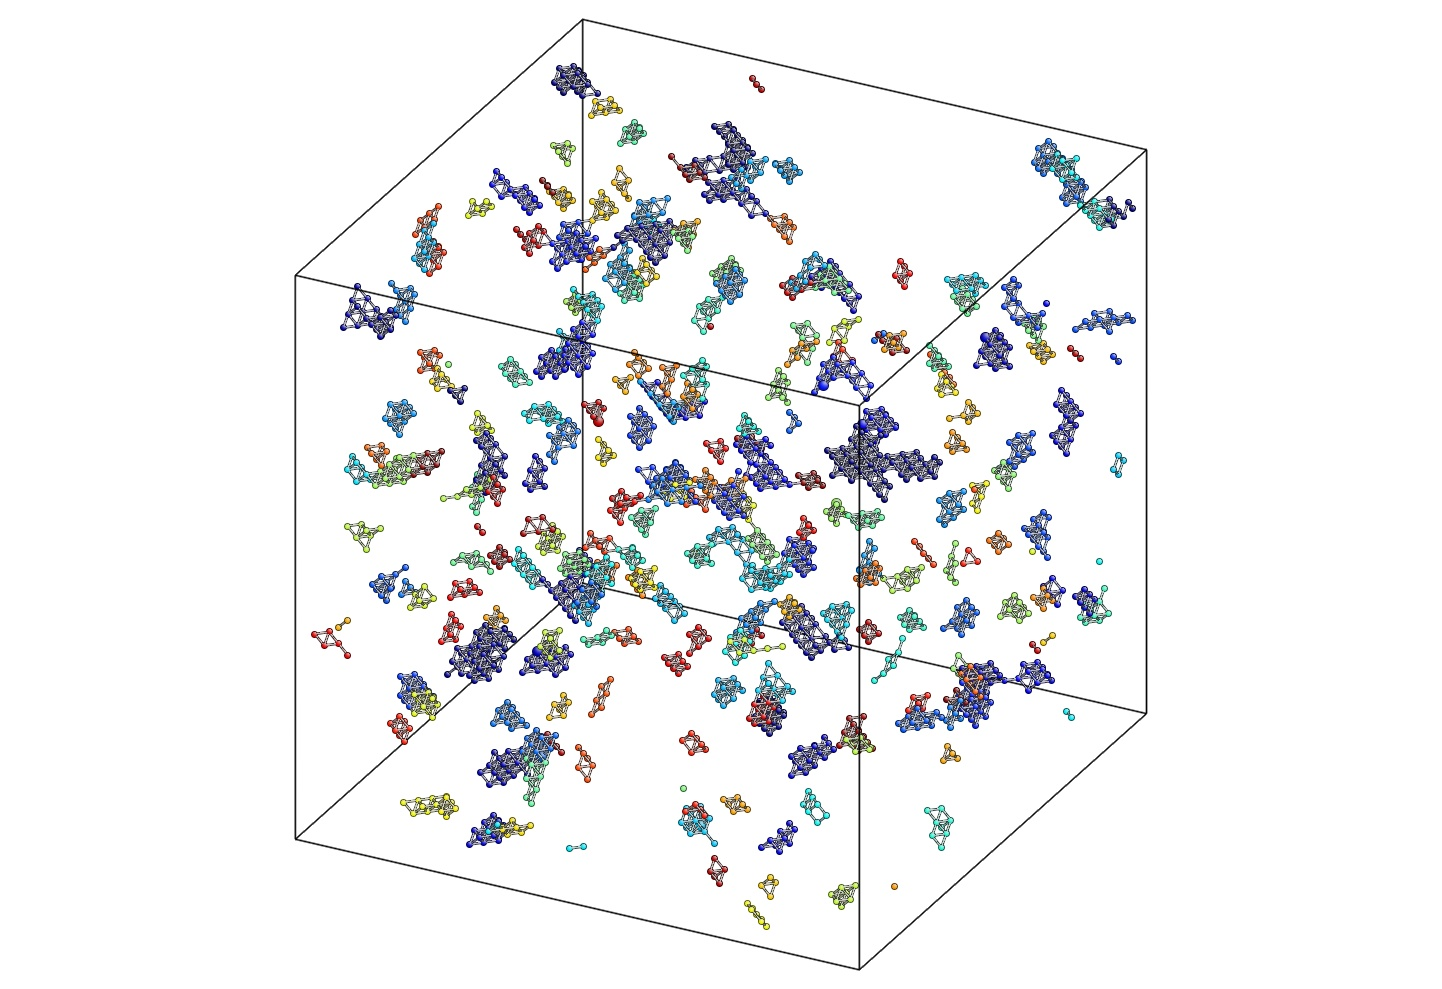
\includegraphics[width=0.32\linewidth]{Chap5/plots/cluster_id_jpg/00000.jpg}}
  \subfigure[$\varepsilon_{Mg-X} = -0.05$, cluster]{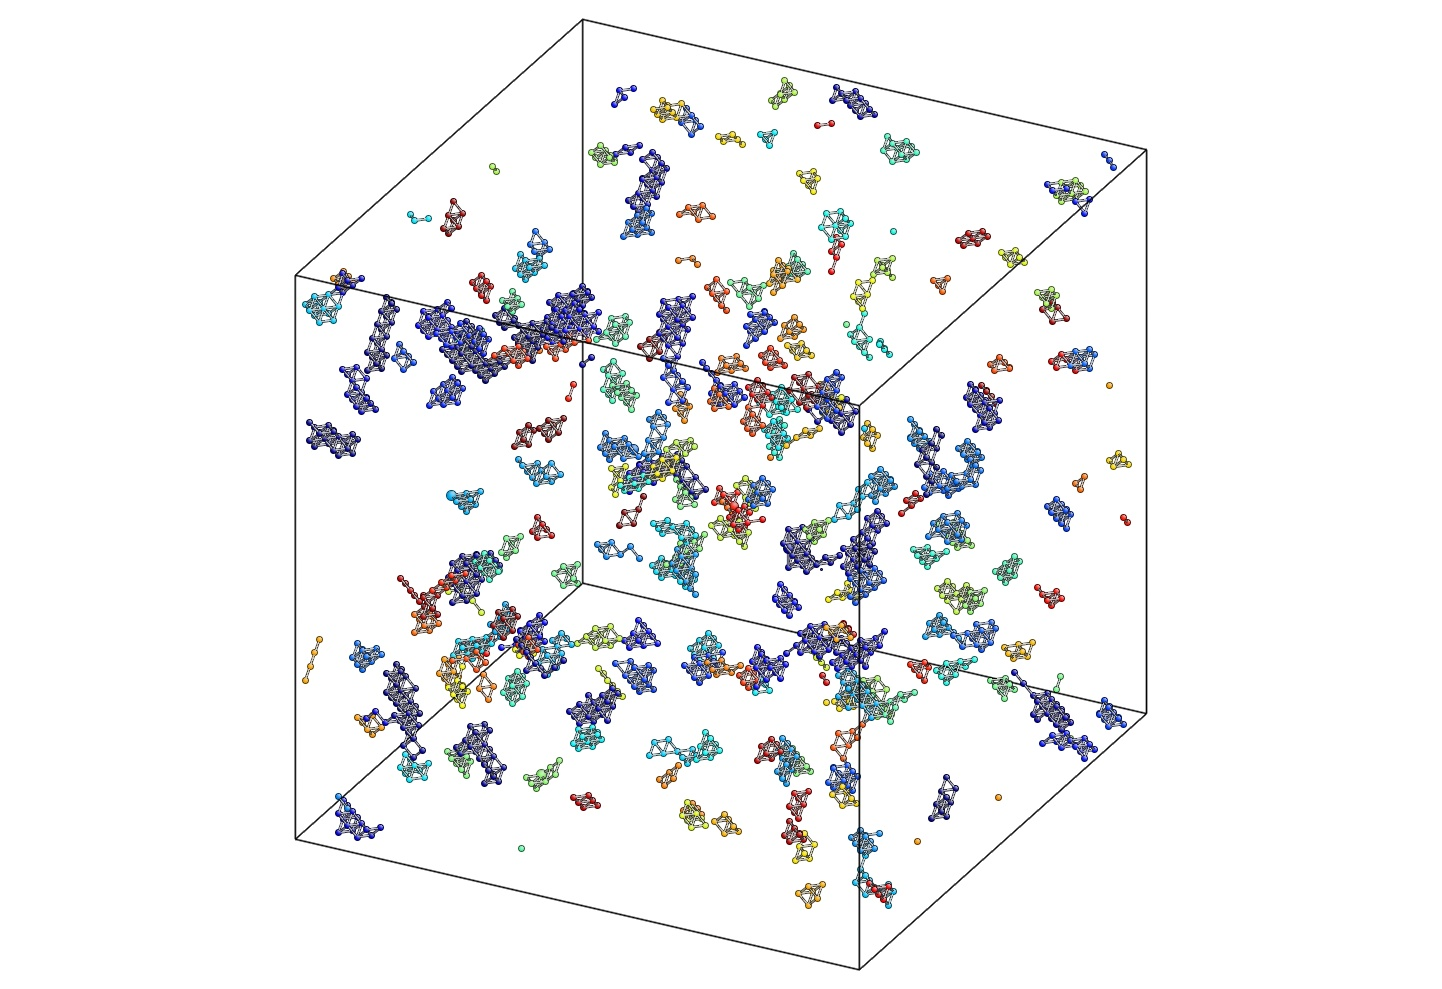
\includegraphics[width=0.49\linewidth]{Chap5/plots/cluster_id_jpg/00004.jpg}} \\
  \subfigure[$\varepsilon_{Mg-X} = 0.05$, species]{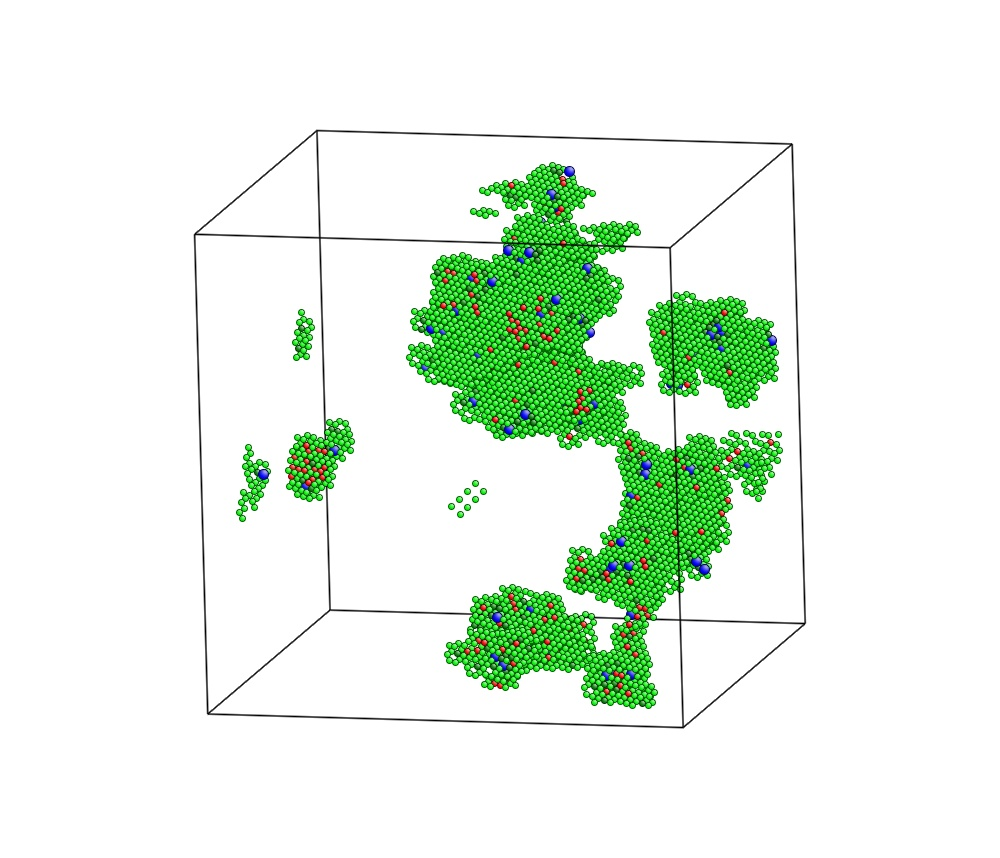
\includegraphics[width=0.49\linewidth]{Chap5/plots/element_jpg/00003.jpg}}
%   \subfigure[control]{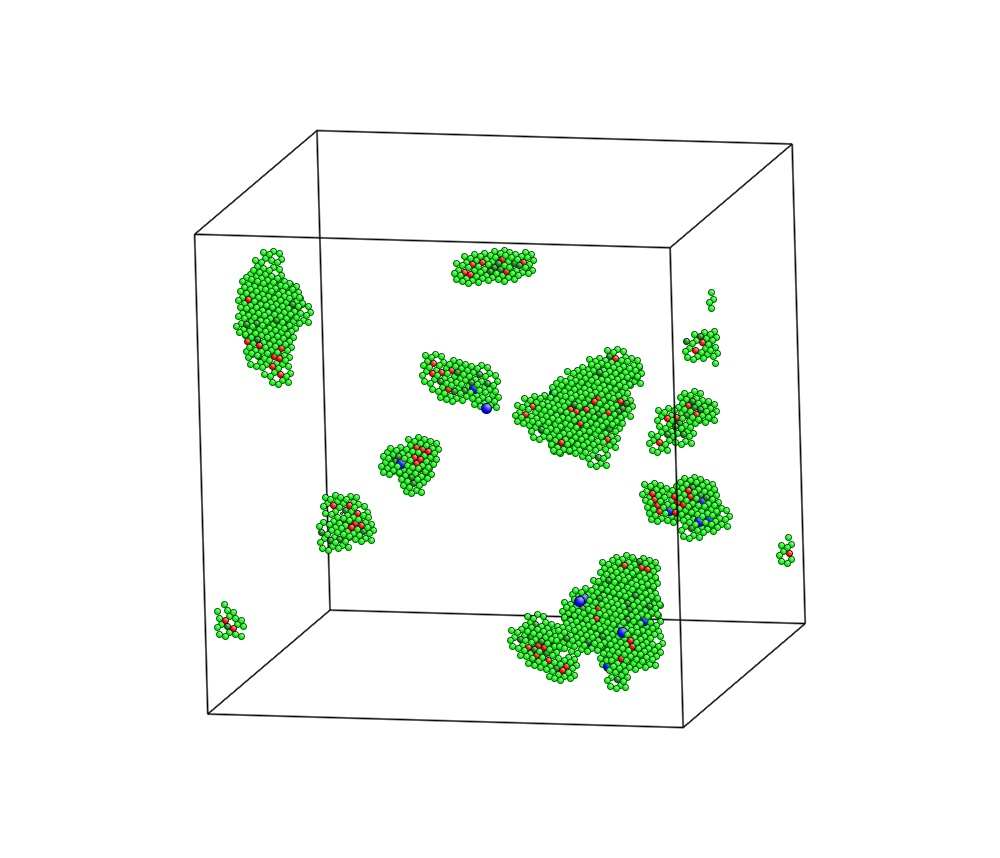
\includegraphics[width=0.32\linewidth]{Chap5/plots/element_jpg/00000.jpg}}
  \subfigure[$\varepsilon_{Mg-X} = -0.05$, species]{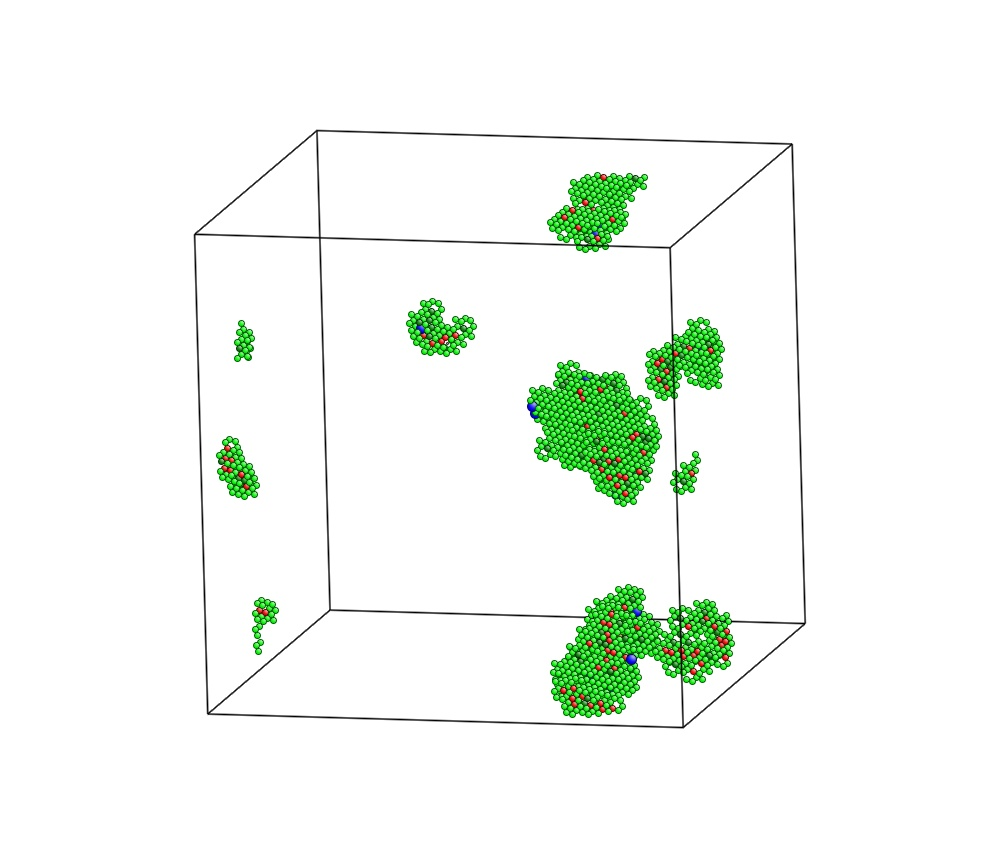
\includegraphics[width=0.49\linewidth]{Chap5/plots/element_jpg/00004.jpg}}
% \caption[Atomistic pictures of 108,000 atoms for $\varepsilon_{Mg-X}$ sensitivity test.]{Atomistic pictures of 108,000 atoms for $\varepsilon_{Mg-X}$ sensitivity test. (a), (d) : $\varepsilon_{Mg-X} = 0.05$, which is setup \#3 in Table \ref{Chap:Al/Vac:tab:pseudo1}. (b), (e) : setup \#0 in Table \ref{Chap:Al/Vac:tab:pseudo1}. (c), (f) : $\varepsilon_{Mg-X} = -0.05$, which is setup \#4 in Table \ref{Chap:Al/Vac:tab:pseudo1}. (a), (b), and (c) are colored by cluster size. The color mapping from dark blue to red is ranked by the cluster size in descending order. (d), (e), and (f) are colored by atom species.  Light green, dark green, red, and blue atoms are Al, Mg, Zn, and pseudo atoms respectively.}
\caption[Atomistic pictures of 108,000 atoms for $\varepsilon_{Mg-X}$ sensitivity test.]{Atomistic pictures of 108,000 atoms for $\varepsilon_{Mg-X}$ sensitivity test. (a), (c) : $\varepsilon_{Mg-X} = 0.05$, which is setup \#3 in Table \ref{Chap:Al/Vac:tab:pseudo1}. (b), (d) : $\varepsilon_{Mg-X} = -0.05$, which is setup \#4 in Table \ref{Chap:Al/Vac:tab:pseudo1}. (a) and (c) are colored by cluster size. The color mapping from dark blue to red is ranked by the cluster size in descending order. (b) and (d) are colored by atom species. Light green, dark green, red, and blue atoms are Al, Mg, Zn, and pseudo atoms respectively. And small gray sticks are bonds between atoms.}
\label{Chap:Al/Vac:fig:sens_Mg}
\end{figure}
\endgroup

\newpage
\begingroup
\begin{figure}[!ht]
  \centering
  \subfigure[$\varepsilon_{Zn-X} = 0.05$, cluster]{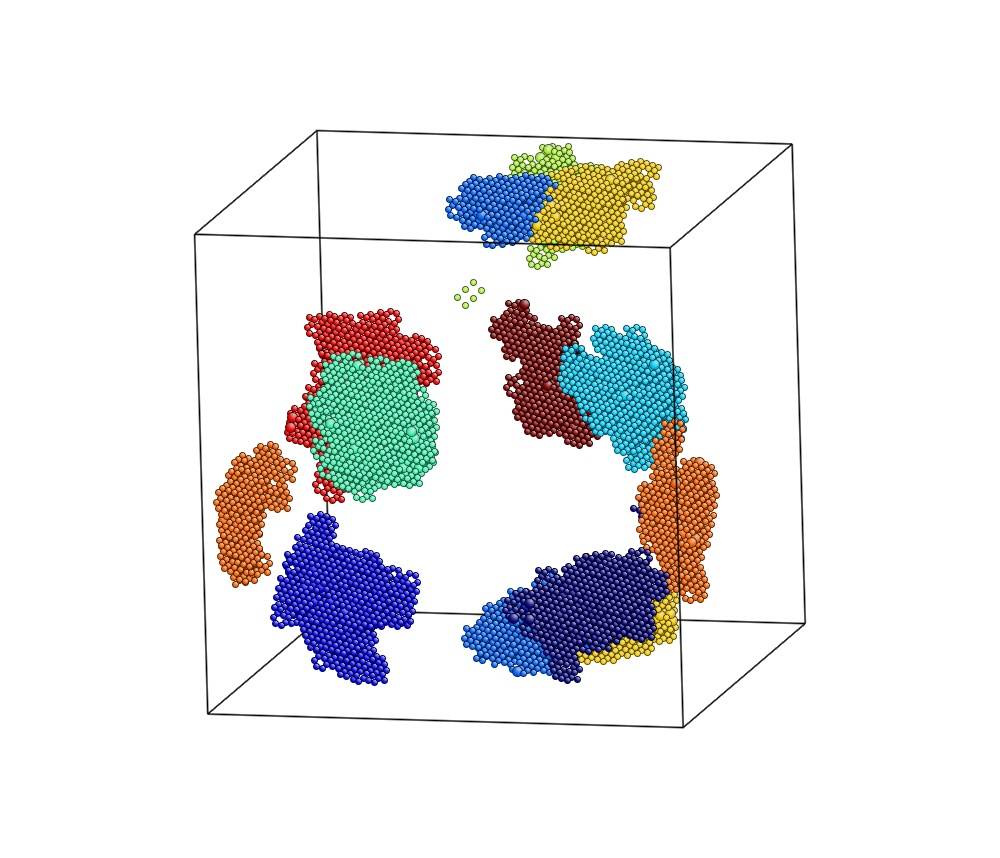
\includegraphics[width=0.49\linewidth]{Chap5/plots/cluster_id_jpg/00005.jpg}}
%   \subfigure[control]{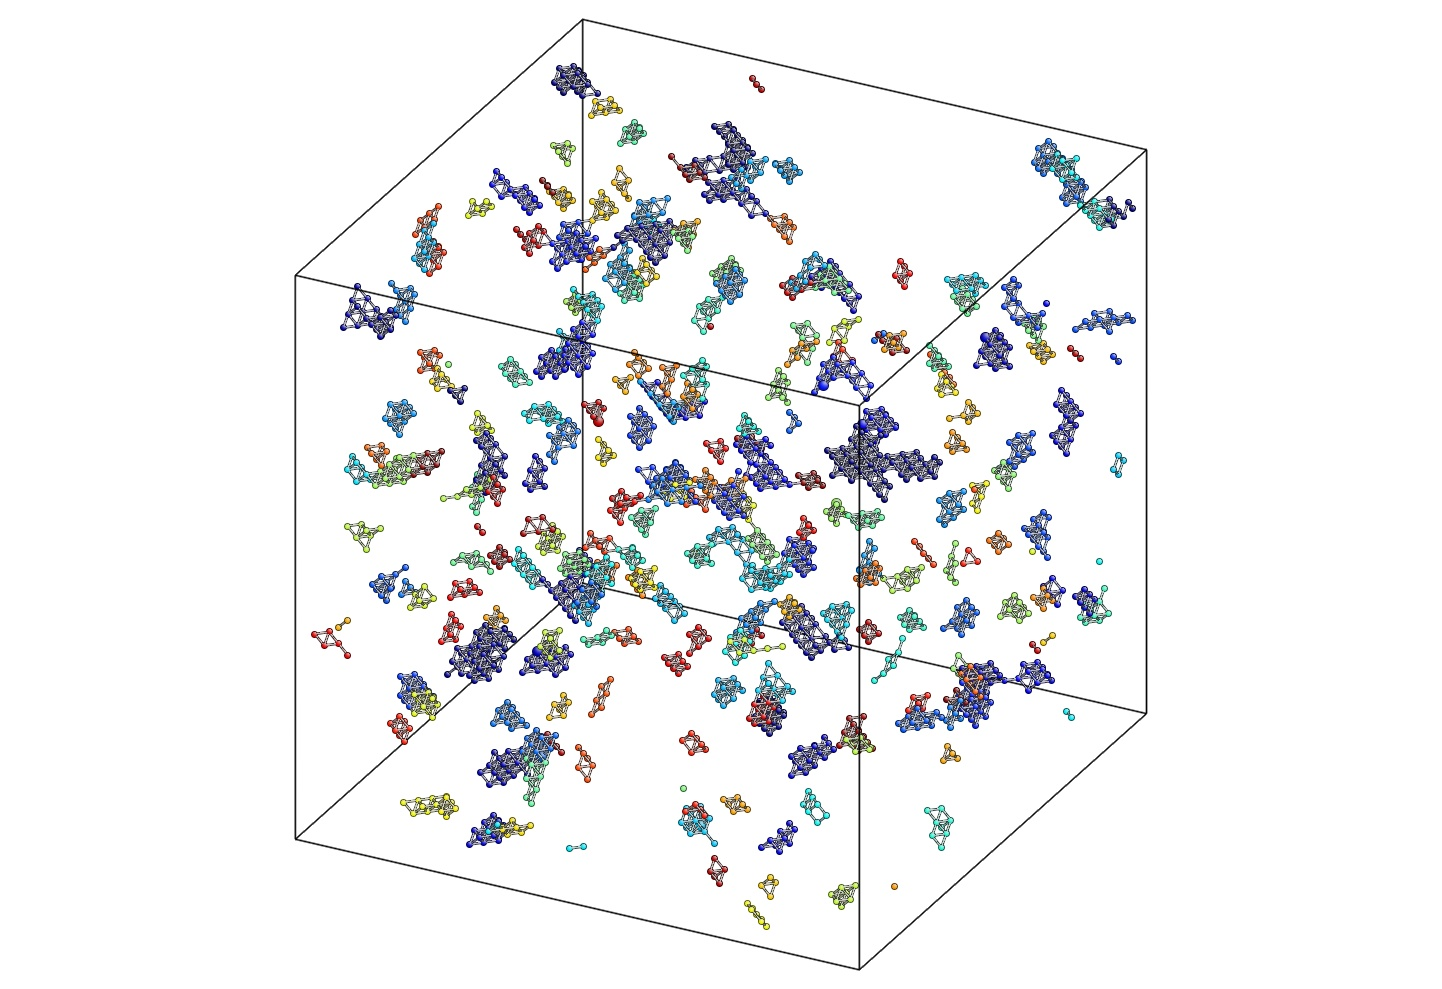
\includegraphics[width=0.32\linewidth]{Chap5/plots/cluster_id_jpg/00000.jpg}}
  \subfigure[$\varepsilon_{Zn-X} = -0.05$, cluster]{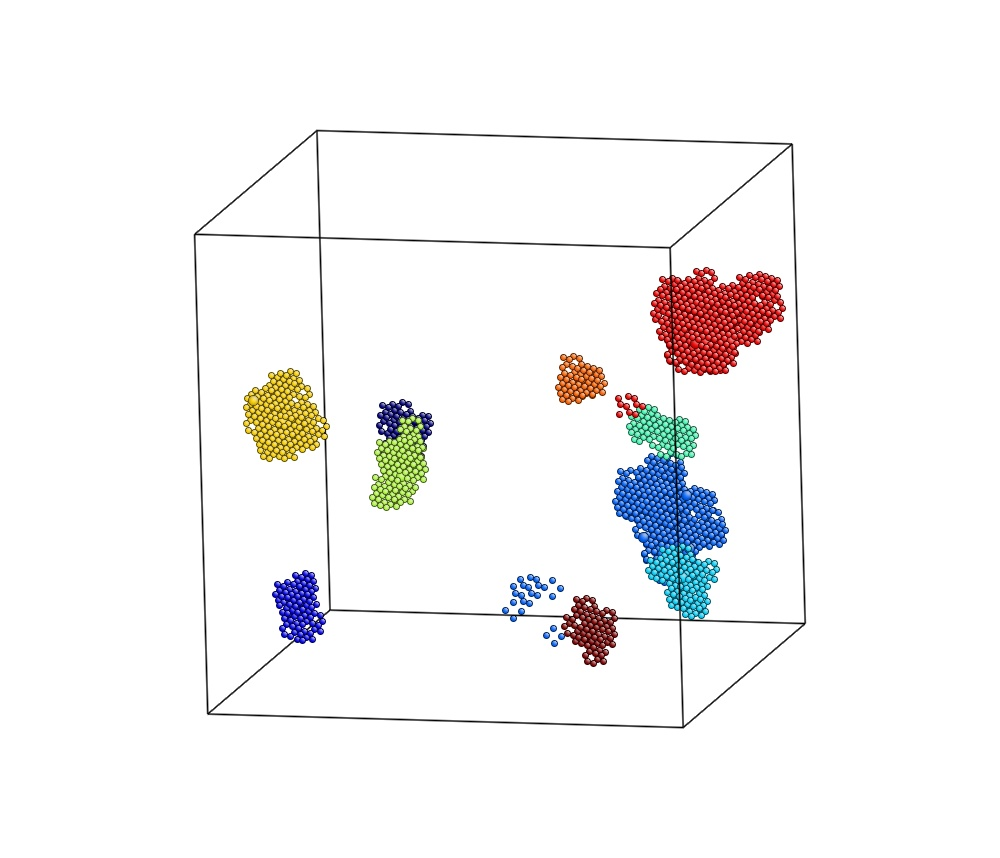
\includegraphics[width=0.49\linewidth]{Chap5/plots/cluster_id_jpg/00006.jpg}} \\
  \subfigure[$\varepsilon_{Zn-X} = 0.05$, species]{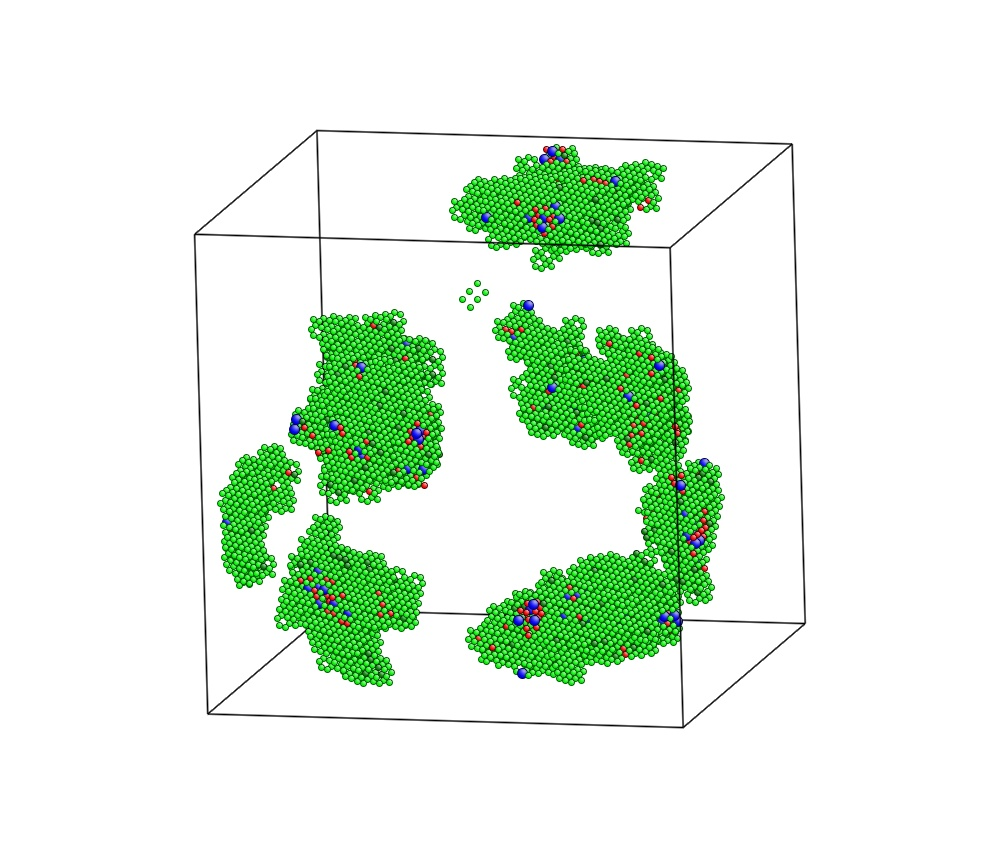
\includegraphics[width=0.49\linewidth]{Chap5/plots/element_jpg/00005.jpg}}
%   \subfigure[control]{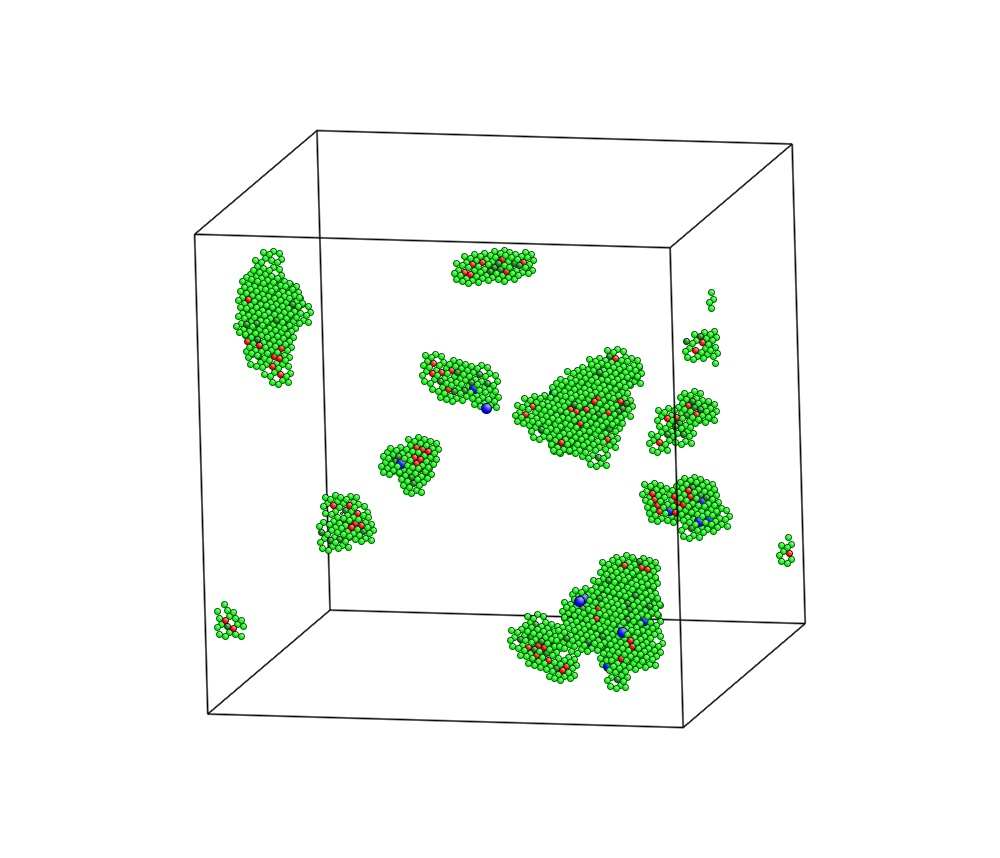
\includegraphics[width=0.32\linewidth]{Chap5/plots/element_jpg/00000.jpg}}
  \subfigure[$\varepsilon_{Zn-X} = -0.05$, species]{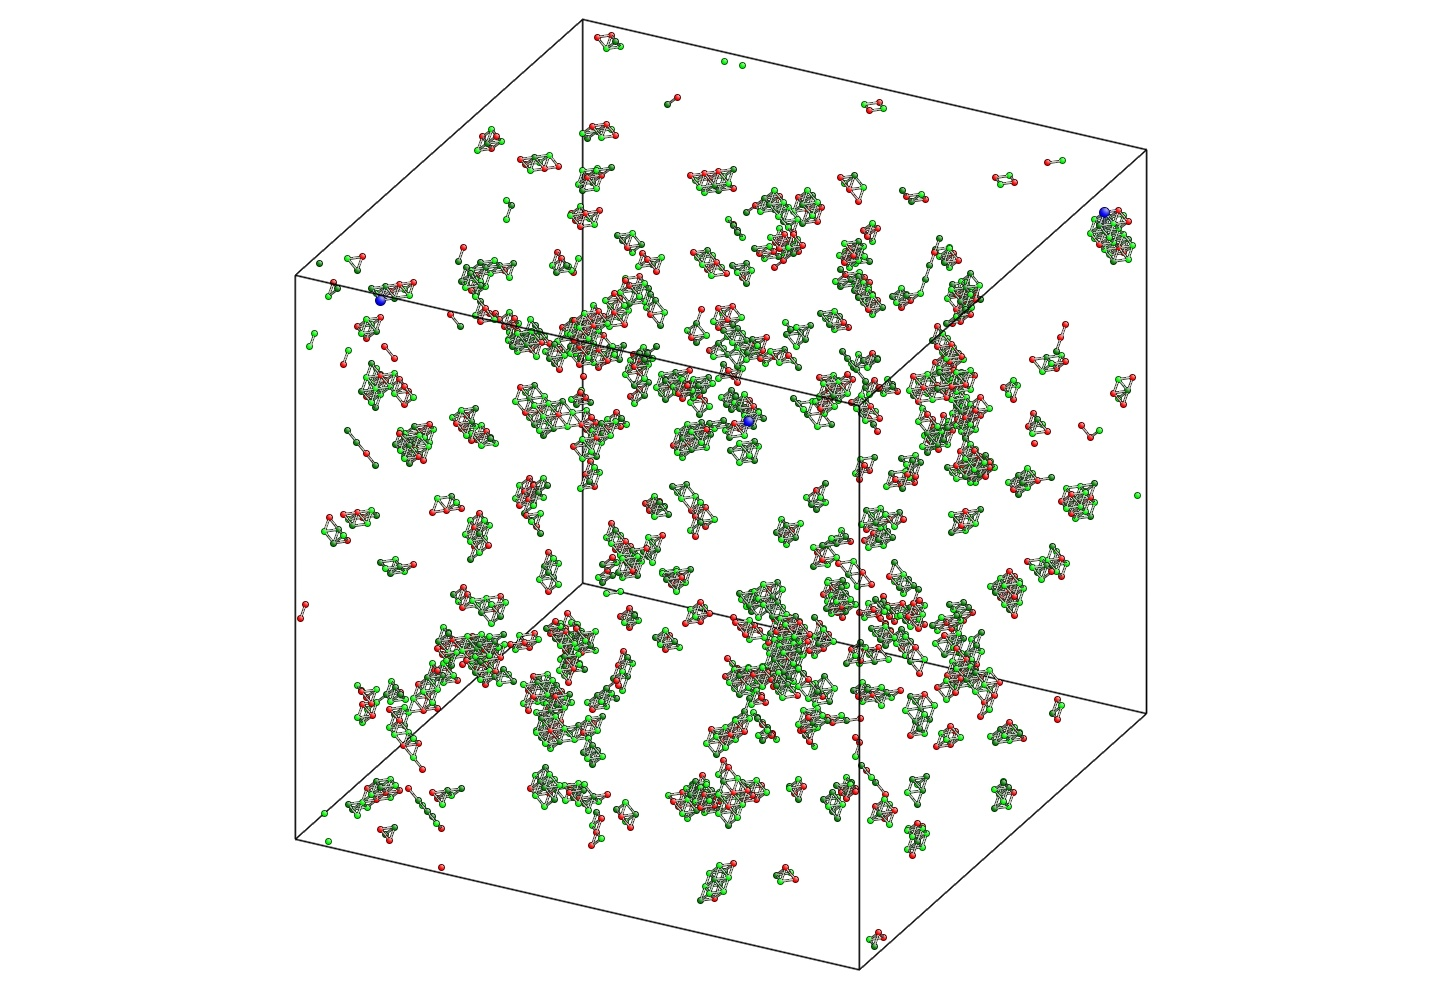
\includegraphics[width=0.49\linewidth]{Chap5/plots/element_jpg/00006.jpg}}
% \caption[Atomistic pictures of 108,000 atoms for $\varepsilon_{Zn-X}$ sensitivity test.]{Atomistic pictures of 108,000 atoms for $\varepsilon_{Zn-X}$ sensitivity test. (a), (d) : $\varepsilon_{Zn-X} = 0.05$, which is setup \#5 in Table \ref{Chap:Al/Vac:tab:pseudo1}. (b), (e) : setup \#0 in Table \ref{Chap:Al/Vac:tab:pseudo1}. (c), (f) : $\varepsilon_{Zn-X} = -0.05$, which is setup \#6 in Table \ref{Chap:Al/Vac:tab:pseudo1}. (a), (b), and (c) are colored by cluster size. The color mapping from dark blue to red is ranked by the cluster size in descending order. (d), (e), and (f) are colored by atom species.  Light green, dark green, red, and blue atoms are Al, Mg, Zn, and pseudo atoms respectively.}
\caption[Atomistic pictures of 108,000 atoms for $\varepsilon_{Zn-X}$ sensitivity test.]{Atomistic pictures of 108,000 atoms for $\varepsilon_{Zn-X}$ sensitivity test. (a), (c) : $\varepsilon_{Zn-X} = 0.05$, which is setup \#5 in Table \ref{Chap:Al/Vac:tab:pseudo1}. (b), (d) : $\varepsilon_{Zn-X} = -0.05$, which is setup \#6 in Table \ref{Chap:Al/Vac:tab:pseudo1}. (a) and (c) are colored by cluster size. The color mapping from dark blue to red is ranked by the cluster size in descending order. (b) and (d) are colored by atom species. Light green, dark green, red, and blue atoms are Al, Mg, Zn, and pseudo atoms respectively. And small gray sticks are bonds between atoms.}
\label{Chap:Al/Vac:fig:sens_Zn}
\end{figure}
\endgroup